% Options for packages loaded elsewhere
\PassOptionsToPackage{unicode}{hyperref}
\PassOptionsToPackage{hyphens}{url}
%
\documentclass[
]{book}
\usepackage{lmodern}
\usepackage{amsmath}
\usepackage{ifxetex,ifluatex}
\ifnum 0\ifxetex 1\fi\ifluatex 1\fi=0 % if pdftex
  \usepackage[T1]{fontenc}
  \usepackage[utf8]{inputenc}
  \usepackage{textcomp} % provide euro and other symbols
  \usepackage{amssymb}
\else % if luatex or xetex
  \usepackage{unicode-math}
  \defaultfontfeatures{Scale=MatchLowercase}
  \defaultfontfeatures[\rmfamily]{Ligatures=TeX,Scale=1}
\fi
% Use upquote if available, for straight quotes in verbatim environments
\IfFileExists{upquote.sty}{\usepackage{upquote}}{}
\IfFileExists{microtype.sty}{% use microtype if available
  \usepackage[]{microtype}
  \UseMicrotypeSet[protrusion]{basicmath} % disable protrusion for tt fonts
}{}
\makeatletter
\@ifundefined{KOMAClassName}{% if non-KOMA class
  \IfFileExists{parskip.sty}{%
    \usepackage{parskip}
  }{% else
    \setlength{\parindent}{0pt}
    \setlength{\parskip}{6pt plus 2pt minus 1pt}}
}{% if KOMA class
  \KOMAoptions{parskip=half}}
\makeatother
\usepackage{xcolor}
\IfFileExists{xurl.sty}{\usepackage{xurl}}{} % add URL line breaks if available
\IfFileExists{bookmark.sty}{\usepackage{bookmark}}{\usepackage{hyperref}}
\hypersetup{
  pdftitle={계층모형 실습},
  pdfauthor={이용희},
  hidelinks,
  pdfcreator={LaTeX via pandoc}}
\urlstyle{same} % disable monospaced font for URLs
\usepackage{color}
\usepackage{fancyvrb}
\newcommand{\VerbBar}{|}
\newcommand{\VERB}{\Verb[commandchars=\\\{\}]}
\DefineVerbatimEnvironment{Highlighting}{Verbatim}{commandchars=\\\{\}}
% Add ',fontsize=\small' for more characters per line
\usepackage{framed}
\definecolor{shadecolor}{RGB}{248,248,248}
\newenvironment{Shaded}{\begin{snugshade}}{\end{snugshade}}
\newcommand{\AlertTok}[1]{\textcolor[rgb]{0.94,0.16,0.16}{#1}}
\newcommand{\AnnotationTok}[1]{\textcolor[rgb]{0.56,0.35,0.01}{\textbf{\textit{#1}}}}
\newcommand{\AttributeTok}[1]{\textcolor[rgb]{0.77,0.63,0.00}{#1}}
\newcommand{\BaseNTok}[1]{\textcolor[rgb]{0.00,0.00,0.81}{#1}}
\newcommand{\BuiltInTok}[1]{#1}
\newcommand{\CharTok}[1]{\textcolor[rgb]{0.31,0.60,0.02}{#1}}
\newcommand{\CommentTok}[1]{\textcolor[rgb]{0.56,0.35,0.01}{\textit{#1}}}
\newcommand{\CommentVarTok}[1]{\textcolor[rgb]{0.56,0.35,0.01}{\textbf{\textit{#1}}}}
\newcommand{\ConstantTok}[1]{\textcolor[rgb]{0.00,0.00,0.00}{#1}}
\newcommand{\ControlFlowTok}[1]{\textcolor[rgb]{0.13,0.29,0.53}{\textbf{#1}}}
\newcommand{\DataTypeTok}[1]{\textcolor[rgb]{0.13,0.29,0.53}{#1}}
\newcommand{\DecValTok}[1]{\textcolor[rgb]{0.00,0.00,0.81}{#1}}
\newcommand{\DocumentationTok}[1]{\textcolor[rgb]{0.56,0.35,0.01}{\textbf{\textit{#1}}}}
\newcommand{\ErrorTok}[1]{\textcolor[rgb]{0.64,0.00,0.00}{\textbf{#1}}}
\newcommand{\ExtensionTok}[1]{#1}
\newcommand{\FloatTok}[1]{\textcolor[rgb]{0.00,0.00,0.81}{#1}}
\newcommand{\FunctionTok}[1]{\textcolor[rgb]{0.00,0.00,0.00}{#1}}
\newcommand{\ImportTok}[1]{#1}
\newcommand{\InformationTok}[1]{\textcolor[rgb]{0.56,0.35,0.01}{\textbf{\textit{#1}}}}
\newcommand{\KeywordTok}[1]{\textcolor[rgb]{0.13,0.29,0.53}{\textbf{#1}}}
\newcommand{\NormalTok}[1]{#1}
\newcommand{\OperatorTok}[1]{\textcolor[rgb]{0.81,0.36,0.00}{\textbf{#1}}}
\newcommand{\OtherTok}[1]{\textcolor[rgb]{0.56,0.35,0.01}{#1}}
\newcommand{\PreprocessorTok}[1]{\textcolor[rgb]{0.56,0.35,0.01}{\textit{#1}}}
\newcommand{\RegionMarkerTok}[1]{#1}
\newcommand{\SpecialCharTok}[1]{\textcolor[rgb]{0.00,0.00,0.00}{#1}}
\newcommand{\SpecialStringTok}[1]{\textcolor[rgb]{0.31,0.60,0.02}{#1}}
\newcommand{\StringTok}[1]{\textcolor[rgb]{0.31,0.60,0.02}{#1}}
\newcommand{\VariableTok}[1]{\textcolor[rgb]{0.00,0.00,0.00}{#1}}
\newcommand{\VerbatimStringTok}[1]{\textcolor[rgb]{0.31,0.60,0.02}{#1}}
\newcommand{\WarningTok}[1]{\textcolor[rgb]{0.56,0.35,0.01}{\textbf{\textit{#1}}}}
\usepackage{longtable,booktabs}
\usepackage{calc} % for calculating minipage widths
% Correct order of tables after \paragraph or \subparagraph
\usepackage{etoolbox}
\makeatletter
\patchcmd\longtable{\par}{\if@noskipsec\mbox{}\fi\par}{}{}
\makeatother
% Allow footnotes in longtable head/foot
\IfFileExists{footnotehyper.sty}{\usepackage{footnotehyper}}{\usepackage{footnote}}
\makesavenoteenv{longtable}
\usepackage{graphicx}
\makeatletter
\def\maxwidth{\ifdim\Gin@nat@width>\linewidth\linewidth\else\Gin@nat@width\fi}
\def\maxheight{\ifdim\Gin@nat@height>\textheight\textheight\else\Gin@nat@height\fi}
\makeatother
% Scale images if necessary, so that they will not overflow the page
% margins by default, and it is still possible to overwrite the defaults
% using explicit options in \includegraphics[width, height, ...]{}
\setkeys{Gin}{width=\maxwidth,height=\maxheight,keepaspectratio}
% Set default figure placement to htbp
\makeatletter
\def\fps@figure{htbp}
\makeatother
\setlength{\emergencystretch}{3em} % prevent overfull lines
\providecommand{\tightlist}{%
  \setlength{\itemsep}{0pt}\setlength{\parskip}{0pt}}
\setcounter{secnumdepth}{5}
\usepackage[onehalfspacing]{setspace}

\usepackage[hangul]{kotex}
\newcommand{\pardiff}[2]{\frac{\partial #1}{\partial #2 }}
\newcommand{\pardiffl}[2]{{\partial #1}/{\partial #2 }}
\newcommand{\pardiffd}[2]{\frac{\partial^2 #1}{\partial #2^t \partial #2 }}
\newcommand{\pardiffdd}[3]{\frac{\partial^2 #1}{\partial #2 \partial #3 }}

\newcommand{\bm}[1]{ \symbf{#1}}

\usepackage{booktabs}
\usepackage{longtable}
\usepackage[bf,singlelinecheck=off]{caption}

%\setmainfont[UprightFeatures={SmallCapsFont=AlegreyaSC-Regular}]{Alegreya}

\usepackage{framed,color}
\definecolor{shadecolor}{RGB}{248,248,248}

\renewcommand{\textfraction}{0.05}
\renewcommand{\topfraction}{0.8}
\renewcommand{\bottomfraction}{0.8}
\renewcommand{\floatpagefraction}{0.75}

\renewenvironment{quote}{\begin{VF}}{\end{VF}}
\let\oldhref\href
\renewcommand{\href}[2]{#2\footnote{\url{#1}}}

\makeatletter
\newenvironment{kframe}{%
\medskip{}
\setlength{\fboxsep}{.8em}
 \def\at@end@of@kframe{}%
 \ifinner\ifhmode%
  \def\at@end@of@kframe{\end{minipage}}%
  \begin{minipage}{\columnwidth}%
 \fi\fi%
 \def\FrameCommand##1{\hskip\@totalleftmargin \hskip-\fboxsep
 \colorbox{shadecolor}{##1}\hskip-\fboxsep
     % There is no \\@totalrightmargin, so:
     \hskip-\linewidth \hskip-\@totalleftmargin \hskip\columnwidth}%
 \MakeFramed {\advance\hsize-\width
   \@totalleftmargin\z@ \linewidth\hsize
   \@setminipage}}%
 {\par\unskip\endMakeFramed%
 \at@end@of@kframe}
\makeatother

\makeatletter

\@ifundefined{Shaded}{
}{\renewenvironment{Shaded}{\begin{kframe}}{\end{kframe}}}
\makeatother

\newenvironment{rmdblock}[1]
  {
  \begin{itemize}
  \renewcommand{\labelitemi}{
    \raisebox{-.7\height}[0pt][0pt]{
      {\setkeys{Gin}{width=3em,keepaspectratio}\includegraphics{images/#1}}
    }
  }
  \setlength{\fboxsep}{1em}
  \begin{kframe}
  \item
  }
  {
  \end{kframe}
  \end{itemize}
  }
  
\newenvironment{rmdnote}
  {\begin{rmdblock}{note}}
  {\end{rmdblock}}
  
\newenvironment{rmdcaution}
  {\begin{rmdblock}{caution}}
  {\end{rmdblock}}
  
\newenvironment{rmdimportant}
  {\begin{rmdblock}{important}}
  {\end{rmdblock}}
  
\newenvironment{rmdtip}
  {\begin{rmdblock}{tip}}
  {\end{rmdblock}}
  
\newenvironment{rmdwarning}
  {\begin{rmdblock}{warning}}
  {\end{rmdblock}}
  


%\usepackage{makeidx}
%\makeindex

\urlstyle{tt}

\usepackage{amsthm}
\makeatletter
 \def\thm@space@setup{%
   \thm@preskip=8pt plus 2pt minus 4pt
   \thm@postskip=\thm@preskip
}
\makeatother

\frontmatter

\usepackage{booktabs}
\usepackage{longtable}
\usepackage{array}
\usepackage{multirow}
\usepackage{wrapfig}
\usepackage{float}
\usepackage{colortbl}
\usepackage{pdflscape}
\usepackage{tabu}
\usepackage{threeparttable}
\usepackage{threeparttablex}
\usepackage[normalem]{ulem}
\usepackage{makecell}
\usepackage{xcolor}
\ifluatex
  \usepackage{selnolig}  % disable illegal ligatures
\fi
\usepackage[]{natbib}
\bibliographystyle{apalike}

\title{계층모형 실습}
\author{이용희}
\date{2021년 5월 11일}

\begin{document}
\maketitle

{
\setcounter{tocdepth}{1}
\tableofcontents
}
\hypertarget{uxc11cuxbb38}{%
\chapter*{서문}\label{uxc11cuxbb38}}
\addcontentsline{toc}{chapter}{서문}

이 책은 계층모형(hierarchical models)에 대한 예제를 통한 실습, 모형을 적합하는 계산방법에 대하여 다루고자 합니다.

\begin{rmdimportant}
이 책에서 사용된 기호, 표기법, 프로그램의 규칙과 쓰임은 다음과 같습니다.

\begin{itemize}
\tightlist
\item
  스칼라(scalar)와 일변량 확률변수는 일반적으로 보통 글씨체의 소문자로 표기한다. 특별한 이유가 있는 경우 대문자로 표시할 것이다.
\item
  벡터, 행렬, 다변량 확률벡터는 굵은 글씨체로 표기한다.\\
\item
  통계 프로그램은 \texttt{R}을 이용하였다. 각 예제에 사용된 \texttt{R} 프로그램은 코드 상자를 열면 나타난다.
\item
  통계 프로그램은 \texttt{R}에 대한 기초는 저자의 홈페이지에 있는 \href{https://ilovedata.github.io/computing/}{안내 사이트}에서 먼저 학습할 것을 권장한다.
\end{itemize}
\end{rmdimportant}

다음은 이 책에서 \texttt{R} 실습을 하기 위하여 필요한 패키지이다.

\begin{verbatim}
library(tidyr)
library(dplyr)
library(ggplot2)
library(knitr)
library(kableExtra)
library(lme4)
library(lmerTest)
library(brms)
library(sas7bdat)
library(sampling)
library(stringr)
library(survey)
library(sae)
\end{verbatim}

\mainmatter

\hypertarget{sleep}{%
\chapter{반복측정자료}\label{sleep}}

\hypertarget{uxac1cuxc694}{%
\section{개요}\label{uxac1cuxc694}}

반복측정자료(longitudinal data, repeated measurements)는 관측단위안에서 여러 개의 관측값을 측정한 자료의 형식을 말한다.

예를 들어 환자가 병원을 여러 번 방문할 때마다 혈압을 측정하였다면 한 명의 환자에서 반복 측정한 자료는 서로 독립이 아니다. 또한 가구조사(household survey)에서 가구원의 경제덕 상태, 건겅 상태 등을 여러 해동안 매년 측정하는 경우가 있는데 이러한 자료를 패널자료(panel data) 또는 longitudinal 자료라고 한다. 이렇게 하나의 관측단위 안에서 반복 측정한 자료들은 서로 독립이 아닌 특징이 있고 자료를 분석하는 경우 이러한 자료들의 종속구조를 고려하는 모형을 사용하는 것이 적절하다.

이렇게 반복측정자료에서 반복자료들의 공분산구조를 설정하는 통계적 방법들은 다양하지만 대표적으로 쉽게 사용할 수 있는 방법이 임의효과를 포함한 혼합모형을 사용하는 방법이다.

\hypertarget{sleepstudy-uxc790uxb8cc}{%
\section{\texorpdfstring{\texttt{sleepstudy} 자료}{sleepstudy 자료}}\label{sleepstudy-uxc790uxb8cc}}

\texttt{lme4} 패키지에 자료인 \texttt{spleepstudy}는 화물트럭 운전사들에 대한 수면부족 현상에 대하여 연구한 자료이다. 18명의 운전자들이 매일 3시간의 수면(부족한 수면)을 하면서
매일 일정한 동작에 대한 반응시간을 10일 동안 반복적으로 측정한 자료이다.
한명의 운전사에게 10일 동안의 반응에 대한 측정자료 10개가 존재하므로 이는 반복측정 자료이며 이러한 10개의 자료는 독립이 아니다.

혼합모형을 적합할 수 있는 \texttt{R} 패키지는 여러 가지 다양한 패키지가 있지만 최대가능도 추정법에 기반한
\texttt{lme4} 패키지를 먼저 이용할 것이다.

일단 자료의 구조를 살펴보자. 반응변수 \texttt{Reaction} 은 반응시간(ms)를 나타내며 설명변수로서 \texttt{Days} 는 날짜(\(t=0,1,2,\dots,9\)), \texttt{Subject} 는 운전자의 고유번호를 나타낸다.

\begin{Shaded}
\begin{Highlighting}[]
\FunctionTok{str}\NormalTok{(sleepstudy)}
\end{Highlighting}
\end{Shaded}

\begin{verbatim}
## 'data.frame':    180 obs. of  3 variables:
##  $ Reaction: num  250 259 251 321 357 ...
##  $ Days    : num  0 1 2 3 4 5 6 7 8 9 ...
##  $ Subject : Factor w/ 18 levels "308","309","310",..: 1 1 1 1 1 1 1 1 1 1 ...
\end{verbatim}

\begin{Shaded}
\begin{Highlighting}[]
\FunctionTok{head}\NormalTok{(sleepstudy,}\AttributeTok{n=}\DecValTok{20}\NormalTok{)}
\end{Highlighting}
\end{Shaded}

\begin{verbatim}
##    Reaction Days Subject
## 1  249.5600    0     308
## 2  258.7047    1     308
## 3  250.8006    2     308
## 4  321.4398    3     308
## 5  356.8519    4     308
## 6  414.6901    5     308
## 7  382.2038    6     308
## 8  290.1486    7     308
## 9  430.5853    8     308
## 10 466.3535    9     308
## 11 222.7339    0     309
## 12 205.2658    1     309
## 13 202.9778    2     309
## 14 204.7070    3     309
## 15 207.7161    4     309
## 16 215.9618    5     309
## 17 213.6303    6     309
## 18 217.7272    7     309
## 19 224.2957    8     309
## 20 237.3142    9     309
\end{verbatim}

\hypertarget{uxac1cuxbcc4uxb2e8uxc704-uxbd84uxc11dno-pooling}{%
\section{개별단위 분석(no pooling)}\label{uxac1cuxbcc4uxb2e8uxc704-uxbd84uxc11dno-pooling}}

각 운전자에 대한 10일 간의 반응속도가 시간에 따라 어떻게 변하는 가를 알아보자. 다음은 10명의 운잔사에 대하여 시간과 반응시간에 대한 산포도를 그리고 각 운전사에 대하여 단순회귀직선을 적합하여 그 결과를 추가한 그림이다.

전반적으로 시간이 지나면서 운전자들의 반응시간이 증가하고 있음을 알 수 있다. 또한 \textbf{개인 별로 반응 시간의 변화와 패턴이 매우 다르다는 것을 알 수 있다.}

\begin{Shaded}
\begin{Highlighting}[]
\FunctionTok{ggplot}\NormalTok{(sleepstudy, }\FunctionTok{aes}\NormalTok{(}\AttributeTok{x=}\NormalTok{Days, }\AttributeTok{y=}\NormalTok{Reaction)) }\SpecialCharTok{+}
     \FunctionTok{geom\_point}\NormalTok{(}\AttributeTok{size=}\FloatTok{0.5}\NormalTok{) }\SpecialCharTok{+}
     \FunctionTok{stat\_smooth}\NormalTok{(}\AttributeTok{method =} \StringTok{"lm"}\NormalTok{,}\AttributeTok{se=}\NormalTok{F,}\AttributeTok{size=}\FloatTok{0.5}\NormalTok{)}\SpecialCharTok{+}
     \FunctionTok{facet\_wrap}\NormalTok{(}\StringTok{"Subject"}\NormalTok{, }\AttributeTok{labeller =}\NormalTok{ label\_both)}\SpecialCharTok{+} 
     \FunctionTok{theme\_bw}\NormalTok{()}
\end{Highlighting}
\end{Shaded}

\begin{verbatim}
## `geom_smooth()` using formula 'y ~ x'
\end{verbatim}

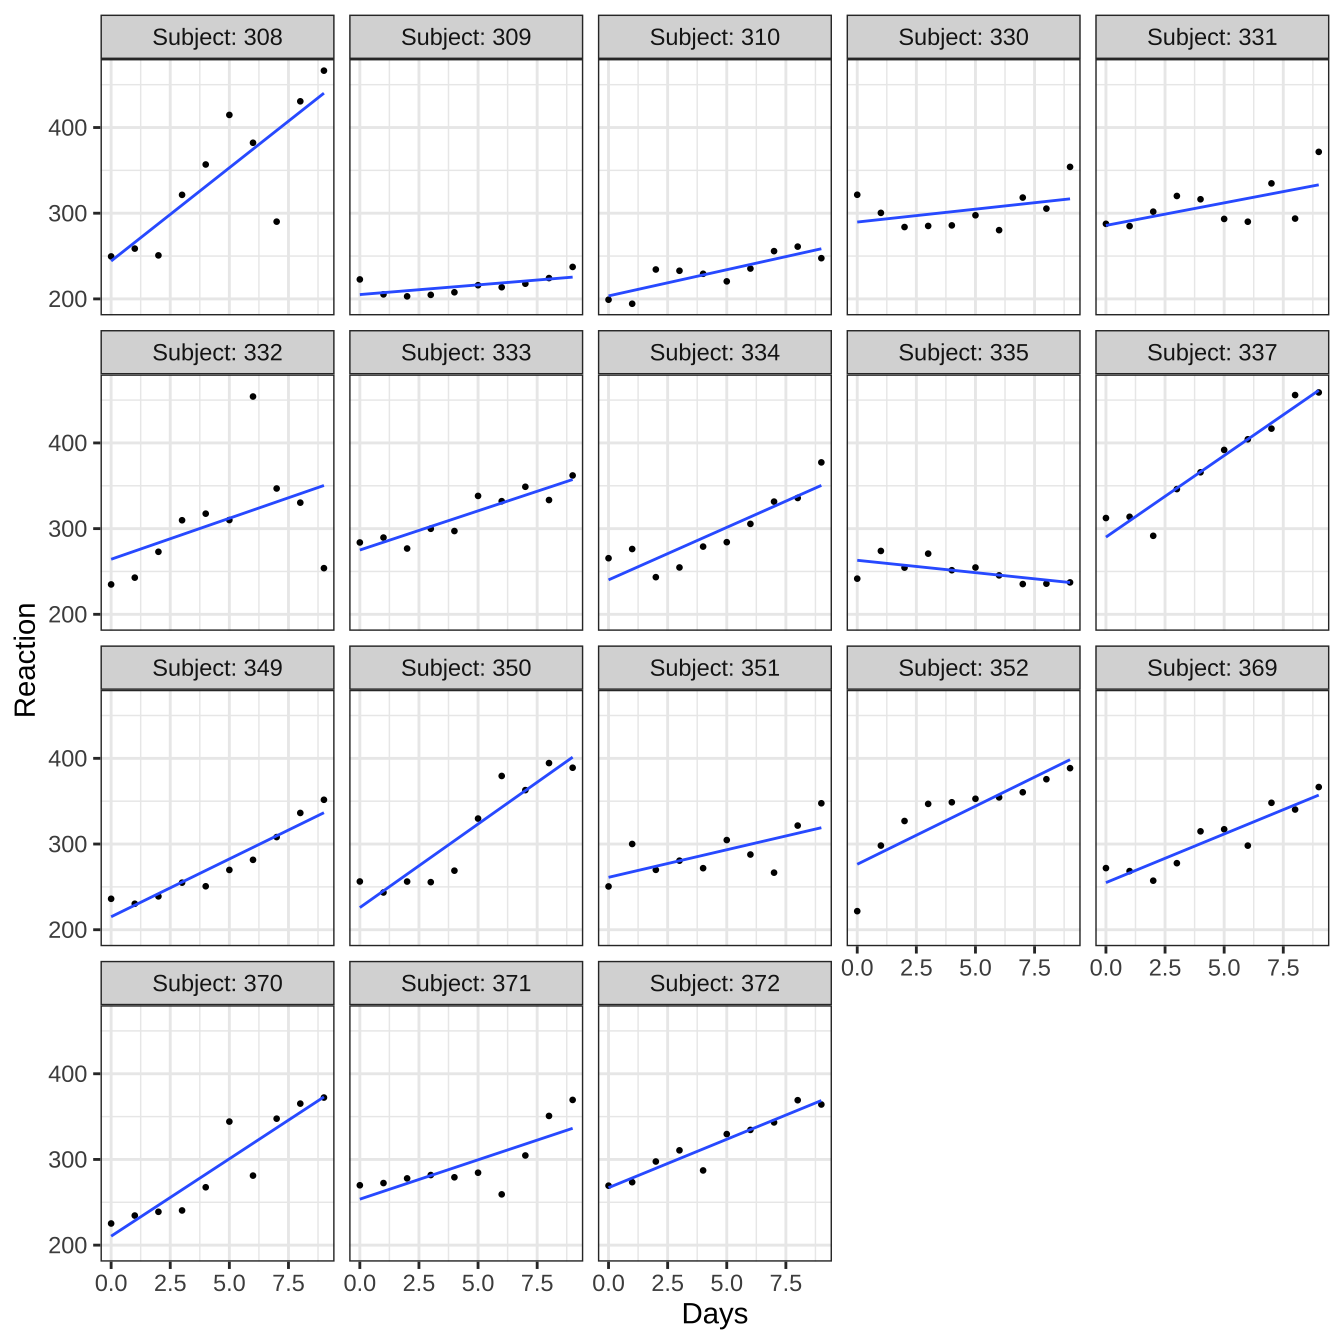
\includegraphics[width=.8\linewidth]{hierarchical_files/figure-latex/ex15-1}

각 \(i\)번째 운전자에 대하여 10일간 측정한 반응속도 \(y_{ij}\)를 시간을 설명변수로 하는 단순 회귀모형을 적합하면 개인별 회귀직선을 다음과 같이 표시할 수 있다.

\begin{equation}
y_{ij} = \beta_{0i} + \beta_{1i} t_j + e_{ij},\quad i=1,2,\dots,18,\quad j=1,2,\dots,10
\label{eq:lmlist1}
\end{equation}

여기서 오차항 \(e_{ij}\)은 서로 독립이며 \(N(0, \sigma^2_e)\)를 따른다고 가정한다.

행렬식으로는 다음과 같이 나타낼 수 있다.

\[  
\bm y_i =\bm X_i \bm \beta_{i} +\bm e_i 
\]

여기서
\[ 
\bm y_i=\begin{bmatrix}
y_{i1} \\
y_{i2} \\
\vdots \\
y_{i,10}
\end{bmatrix},~ \bm X_i =
\begin{bmatrix}
1 & 0 \\
1 & 1 \\
\vdots & \vdots  \\
1 & 9 
\end{bmatrix}, \bm \beta_i=
\begin{bmatrix}
\beta_{0i} \\
\beta_{1i} \\
\end{bmatrix}, \bm e_i= 
\begin{bmatrix}
e_{i1} \\
e_{i2} \\
\vdots \\
e_{i,10}
\end{bmatrix}
\]

위의 식에서 \(\beta_{0i}\)와 \(\beta_{1i}\)는 \(i\)번째 운전사의 반응속도를 설명내는 회귀직선의 절편과 기울기이다. 절편 \(\beta_{0i}\)는 실험 시작때 반응속도를 의미하고 기울기 \(\beta_{1i}\)는 실험이 진행되는 동안 반응속도가 어떻게 변하는 지 변화의 방향과 크기를 보여준다.

함수 \texttt{lmList}를 아래와 같이 이용하면 식 \eqref{eq:lmlist1} 을 각 운전사마다 적합시켜 각각의 절편과 기울기를 구할 수 있다.

함수 \texttt{lmList}에서 모형식 \texttt{Reaction\ \textasciitilde{}\ Days\ \textbar{}\ Subject}은 각 \texttt{Subject} 별로 반응변수를 \texttt{Reaction}으로 하고 설명변수를 \texttt{Days}로 하는 단순회귀모형을 적합하라는 의미이다.

\begin{Shaded}
\begin{Highlighting}[]
\NormalTok{lmf1 }\OtherTok{\textless{}{-}} \FunctionTok{lmList}\NormalTok{(Reaction }\SpecialCharTok{\textasciitilde{}}\NormalTok{ Days }\SpecialCharTok{|}\NormalTok{ Subject, sleepstudy)}
\NormalTok{lmf1}
\end{Highlighting}
\end{Shaded}

\begin{verbatim}
## Call: lmList(formula = Reaction ~ Days | Subject, data = sleepstudy) 
## Coefficients:
##     (Intercept)      Days
## 308    244.1927 21.764702
## 309    205.0549  2.261785
## 310    203.4842  6.114899
## 330    289.6851  3.008073
## 331    285.7390  5.266019
## 332    264.2516  9.566768
## 333    275.0191  9.142045
## 334    240.1629 12.253141
## 335    263.0347 -2.881034
## 337    290.1041 19.025974
## 349    215.1118 13.493933
## 350    225.8346 19.504017
## 351    261.1470  6.433498
## 352    276.3721 13.566549
## 369    254.9681 11.348109
## 370    210.4491 18.056151
## 371    253.6360  9.188445
## 372    267.0448 11.298073
## 
## Degrees of freedom: 180 total; 144 residual
## Residual standard error: 25.59182
\end{verbatim}

\begin{Shaded}
\begin{Highlighting}[]
\FunctionTok{cor}\NormalTok{(}\FunctionTok{coef}\NormalTok{(lmf1))}
\end{Highlighting}
\end{Shaded}

\begin{verbatim}
##             (Intercept)       Days
## (Intercept)   1.0000000 -0.1375534
## Days         -0.1375534  1.0000000
\end{verbatim}

\begin{Shaded}
\begin{Highlighting}[]
\FunctionTok{plot}\NormalTok{(}\FunctionTok{coef}\NormalTok{(lmf1),}\AttributeTok{main=}\StringTok{"intercepts and slopes on drivers: sleep study "}\NormalTok{)}
\end{Highlighting}
\end{Shaded}

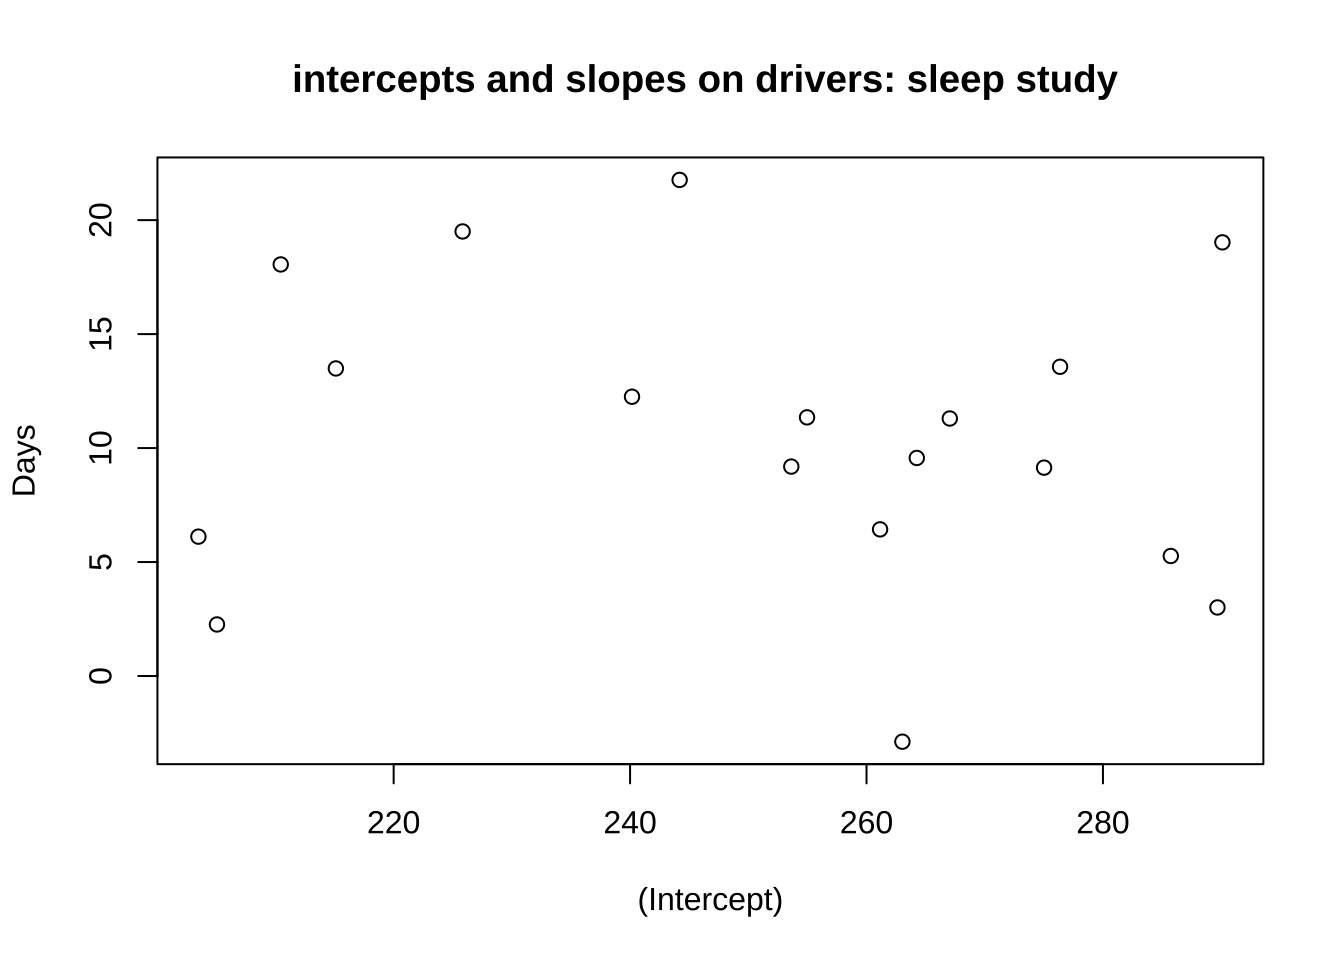
\includegraphics[width=.8\linewidth]{hierarchical_files/figure-latex/ex16-1}

18개의 절편과 기울기는 큰 상관관계는 없는것으로 보이지만 약한 음의 상관계수가 나타났다.

절편과 기울기에 대한 분포를 보기 위하여 상자그림을 그려보면 평균을 중심으로 대칭인 분포를 보이고 있다.

\begin{Shaded}
\begin{Highlighting}[]
\FunctionTok{boxplot}\NormalTok{(}\FunctionTok{coef}\NormalTok{(lmf1)[}\DecValTok{1}\NormalTok{])}
\FunctionTok{title}\NormalTok{(}\StringTok{\textquotesingle{}boxplot for intercepts\textquotesingle{}}\NormalTok{)}
\end{Highlighting}
\end{Shaded}

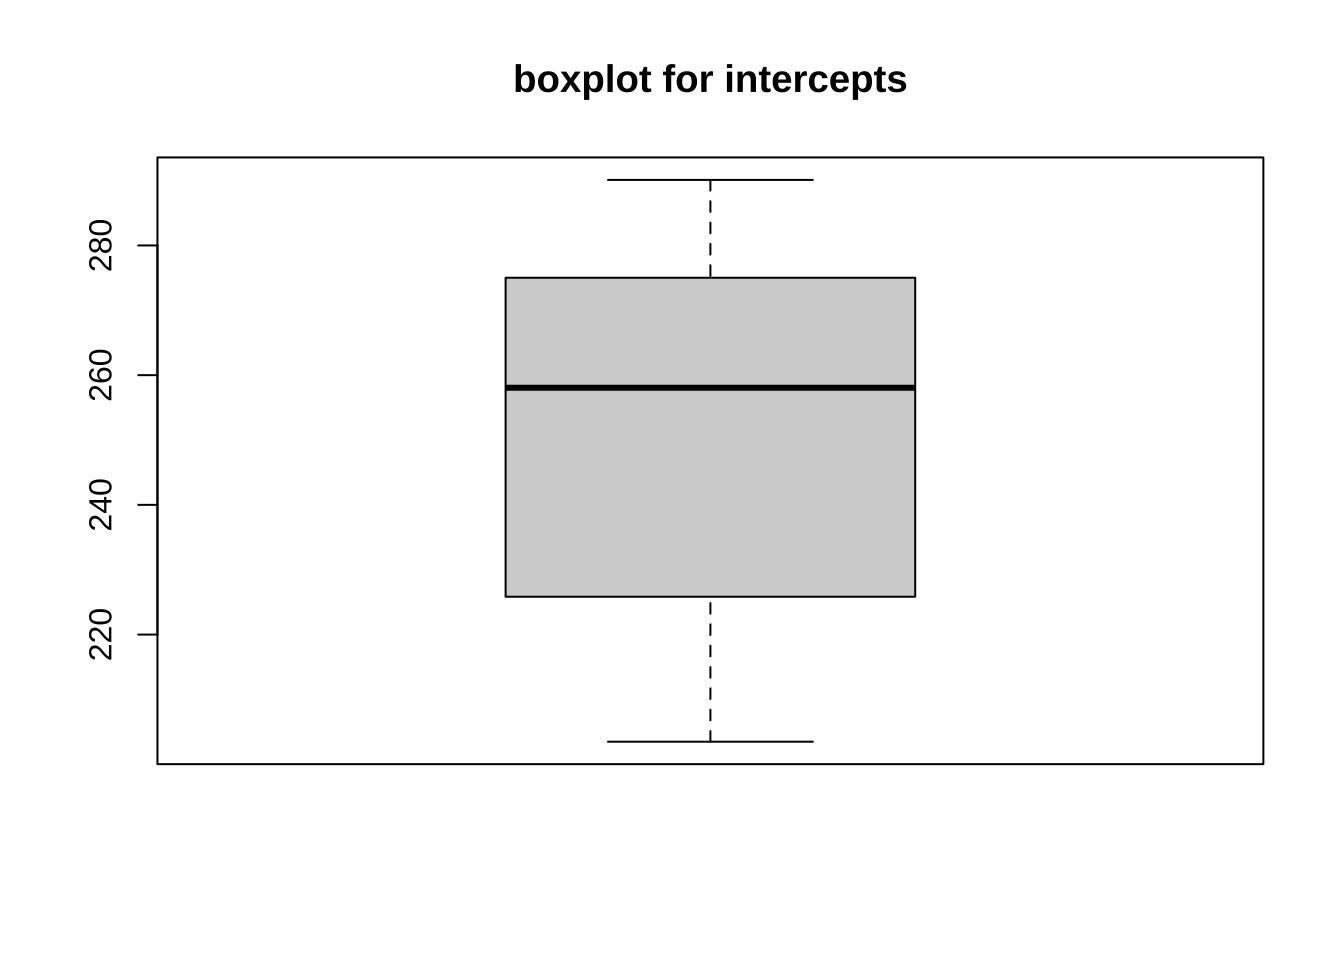
\includegraphics[width=.8\linewidth]{hierarchical_files/figure-latex/box-1}

\begin{Shaded}
\begin{Highlighting}[]
\FunctionTok{boxplot}\NormalTok{(}\FunctionTok{coef}\NormalTok{(lmf1)[}\DecValTok{2}\NormalTok{])}
\FunctionTok{title}\NormalTok{(}\StringTok{\textquotesingle{}boxplot for slopes\textquotesingle{}}\NormalTok{)}
\end{Highlighting}
\end{Shaded}

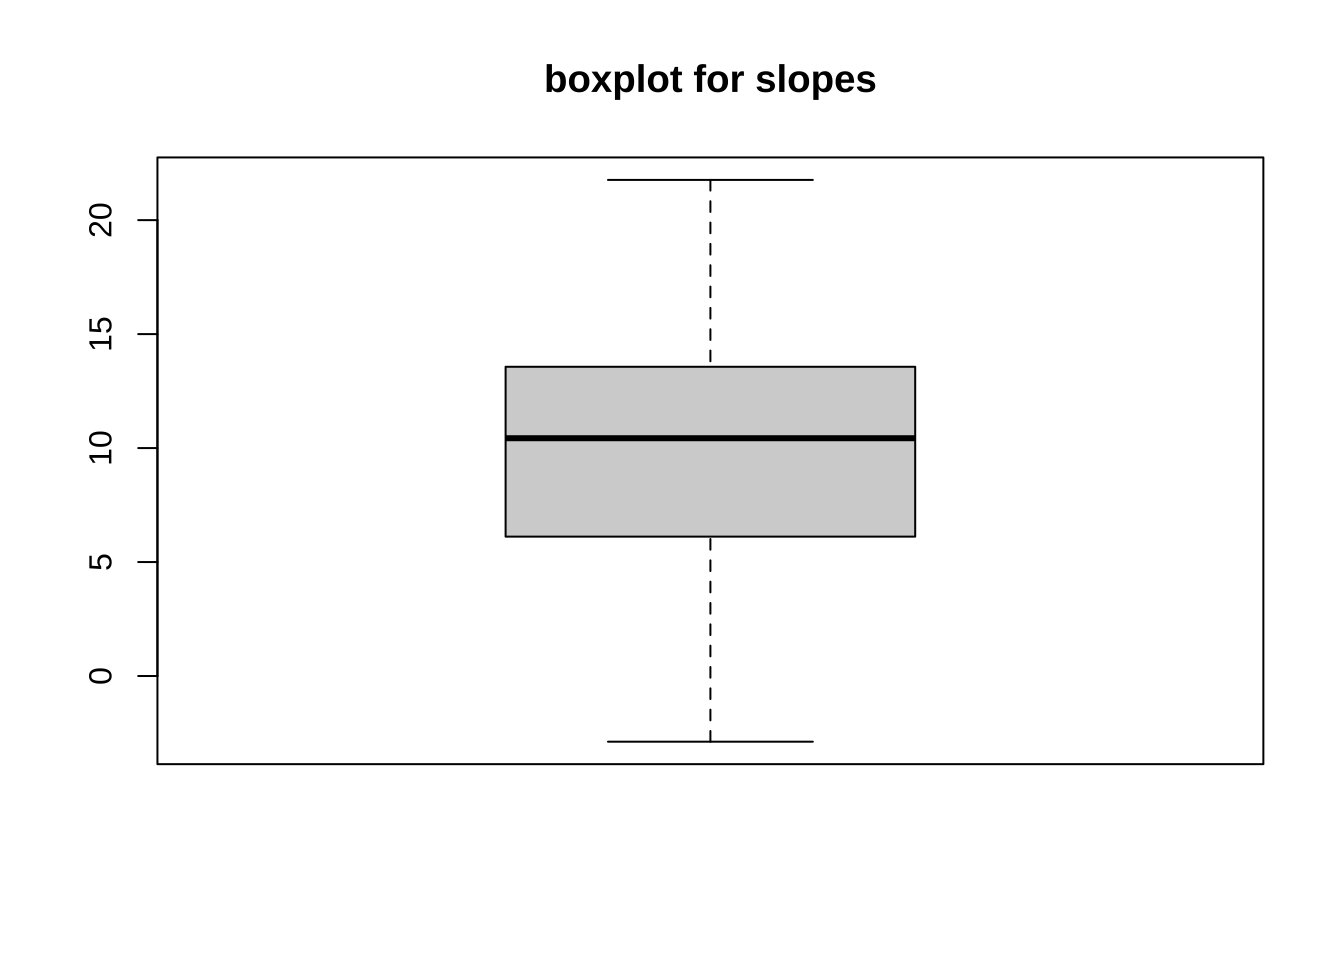
\includegraphics[width=.8\linewidth]{hierarchical_files/figure-latex/box-2}

\hypertarget{uxd1b5uxd569-uxbd84uxc11d-complete-pooling}{%
\section{통합 분석 (complete pooling)}\label{uxd1b5uxd569-uxbd84uxc11d-complete-pooling}}

이제 각 운전사에 대하여 회귀식을 따로 적합하지 않고 전체 운전사들의 자료를 모두 합쳐서 하나의 회귀식을 고려할 수 있다. 개체의 특성을 반영하는 모형이 아닌 \textbf{전체 집단에 대한 평균적인 모형(population model)}을 고려하는 것이다.

\begin{equation} 
y_{ij} = \beta_0 + \beta_1 t_j + e_{ij} ,\quad i=1,2\dots,18,  j=1,2, \dots, 10 
\label{eq:popmodel}
\end{equation}

여기서 오차항은 서로 독립이며 \(N(0, \sigma^2_e)\)를 따른다고 가정한다.

모형 \eqref{eq:popmodel}은 운전자의 특성을 고려하지 않고 전체 운전사 집단의 관측값에 기반한 모형으로서 시간에 따른 반응시간에 대한 관계를 모집단의 평균적 함수 관계를 파악하는 모형이라고 할 수 있다.

\begin{Shaded}
\begin{Highlighting}[]
\NormalTok{lmpop }\OtherTok{\textless{}{-}} \FunctionTok{lm}\NormalTok{(Reaction }\SpecialCharTok{\textasciitilde{}}\NormalTok{ Days, sleepstudy)}
\FunctionTok{summary}\NormalTok{(lmpop)}
\end{Highlighting}
\end{Shaded}

\begin{verbatim}
## 
## Call:
## lm(formula = Reaction ~ Days, data = sleepstudy)
## 
## Residuals:
##      Min       1Q   Median       3Q      Max 
## -110.848  -27.483    1.546   26.142  139.953 
## 
## Coefficients:
##             Estimate Std. Error t value Pr(>|t|)    
## (Intercept)  251.405      6.610  38.033  < 2e-16 ***
## Days          10.467      1.238   8.454 9.89e-15 ***
## ---
## Signif. codes:  0 '***' 0.001 '**' 0.01 '*' 0.05 '.' 0.1 ' ' 1
## 
## Residual standard error: 47.71 on 178 degrees of freedom
## Multiple R-squared:  0.2865, Adjusted R-squared:  0.2825 
## F-statistic: 71.46 on 1 and 178 DF,  p-value: 9.894e-15
\end{verbatim}

아래 그림에서 굵은 선은 모집단의 평균적 함수 관계를 나타나는 모형 \eqref{eq:popmodel}을 적합한 결과이며 점선은 개별 운전사의 자료를 적합한 모형 \eqref{eq:lmlist1} 을 나타낸 그림이다.

\begin{Shaded}
\begin{Highlighting}[]
\FunctionTok{with}\NormalTok{(sleepstudy, }\FunctionTok{plot}\NormalTok{(Days, Reaction,}\AttributeTok{main=}\StringTok{"Population and individual regression lines"}\NormalTok{))}
\FunctionTok{abline}\NormalTok{(}\AttributeTok{a=}\FunctionTok{coef}\NormalTok{(lmpop)[}\DecValTok{1}\NormalTok{], }\AttributeTok{b=}\FunctionTok{coef}\NormalTok{(lmpop)[}\DecValTok{2}\NormalTok{],}\AttributeTok{lwd=}\DecValTok{3}\NormalTok{)}
\ControlFlowTok{for}\NormalTok{ ( i }\ControlFlowTok{in} \DecValTok{1}\SpecialCharTok{:}\DecValTok{18}\NormalTok{ ) \{}
\NormalTok{  xx }\OtherTok{\textless{}{-}} \FunctionTok{as.numeric}\NormalTok{(}\FunctionTok{coef}\NormalTok{(lmf1)[i,])}
\FunctionTok{abline}\NormalTok{(}\AttributeTok{a=}\NormalTok{xx[}\DecValTok{1}\NormalTok{],}\AttributeTok{b=}\NormalTok{xx[}\DecValTok{2}\NormalTok{], }\AttributeTok{lty=}\DecValTok{2}\NormalTok{)}
\NormalTok{\}}
\end{Highlighting}
\end{Shaded}

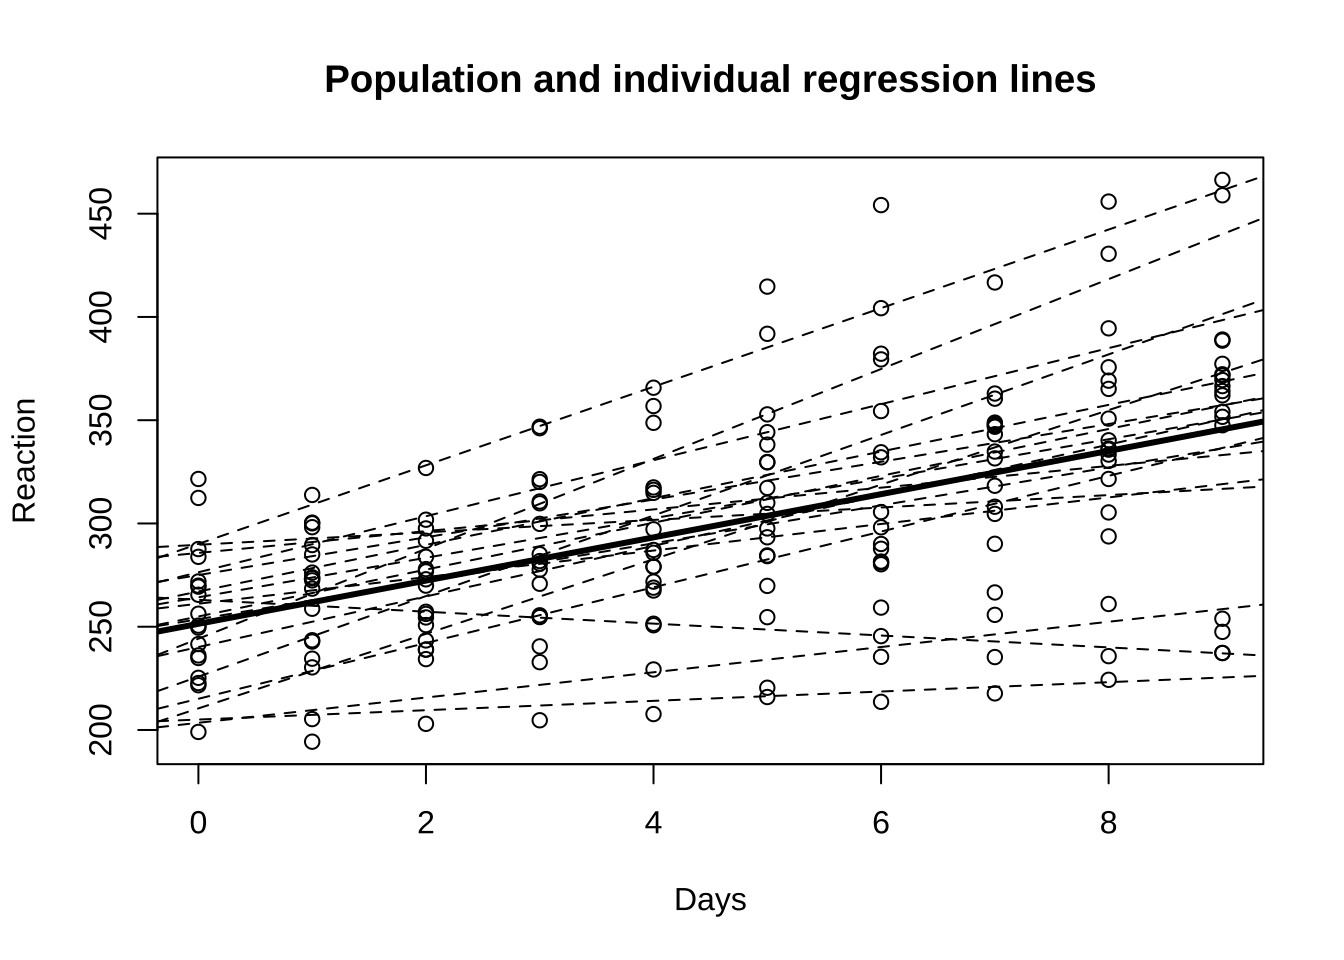
\includegraphics{hierarchical_files/figure-latex/unnamed-chunk-3-1.pdf}

이제 각 운전사에 대하여 개체별로 적합한 회귀식의 계수들\((\hat \beta_{0i}, \hat \beta_{1i})\) 와 전체집단에 적한한 회귀식의 계수 \((\hat \beta_{0}, \hat \beta_{1})\)의 관계를 보면 개체별로 회귀 계수들의 평균이 전체에 적용한 모형의 계수와 매우 가까운 사실을 알 수 있다.

\[ 
\frac{\sum_{i=1}^n \hat \beta_{0i}}{n} \approx \hat \beta_{0}, \quad  \frac{\sum_{i=1}^n \hat \beta_{1i}}{n} \approx \hat \beta_{1}
\]

\begin{Shaded}
\begin{Highlighting}[]
\FunctionTok{apply}\NormalTok{(}\FunctionTok{coef}\NormalTok{(lmf1),}\DecValTok{2}\NormalTok{,mean)}
\end{Highlighting}
\end{Shaded}

\begin{verbatim}
## (Intercept)        Days 
##   251.40510    10.46729
\end{verbatim}

\begin{Shaded}
\begin{Highlighting}[]
\FunctionTok{coef}\NormalTok{(lmpop)}
\end{Highlighting}
\end{Shaded}

\begin{verbatim}
## (Intercept)        Days 
##   251.40510    10.46729
\end{verbatim}

\hypertarget{uxc120uxd615-uxd63cuxd569uxbaa8uxd615partial-pooling}{%
\section{선형 혼합모형(partial pooling)}\label{uxc120uxd615-uxd63cuxd569uxbaa8uxd615partial-pooling}}

\hypertarget{uxc784uxc758uxacc4uxc218uxbaa8uxd615}{%
\subsection{임의계수모형}\label{uxc784uxc758uxacc4uxc218uxbaa8uxd615}}

앞 절의 모형과 분석에서 알 수 있듯이 한 개체에 대하여 여러 개의 관측값을 측정한 자료에 회귀방정식을 각각 적합시켜보고 또한 개체의 특성을 고려하지않은 전체 모형을 적합해보면 다음과 같은 두 가지 결과를 볼 수 있다.

\begin{itemize}
\tightlist
\item
  각 개체별 회귀식은 개인의 특성을 반영한다. 즉, 개체에 따라 시간에 따른 반응시간의 변화가 다르게 나타난다.
\item
  하지만 개인별로 볼 때도 전체적으로는 시간에 따라서 반응시간이 증가하는 경향이 있음을 알 수 있다.
\item
  전체 자료에 적합한 모형을 보면 개인별로 적합한 모형의 공통적인 성격, 즉 시간에 따른 반응시간의 증가를 알 수 있다.
\item
  이러한 결과를 보고 각 개인의 변화는 전체적인 변화를 따르면서 각 개인의 특성이 반영되었다고 가정할 수 있다.
\end{itemize}

위에서 논의하였듯이 전체적인 경향과 게인의 특성을 동시에 고려할 수 있는 모형이 생각할 수 있고 이러한 모형이 다음과 같은 모형이다.

\begin{equation} 
y_{ij} = (\beta_0 + b_{0i}) + (\beta_1 + b_{1i}) t_j + e_{ij} 
\label{eq:repeat}
\end{equation}

모형 \eqref{eq:repeat} 는 절편과 기울기가 두 개의 구성 요소로 더해져서 표현된다.

기울기는 \(\beta_1+b_{1i}\)로서 나타내어지며 \(\beta_1\)은 모집단이 가지는 공통적인 경향을 반영하는 모수이고 \(b_{1i}\)는 \(i\) 번째 개체의 특성을 반영한 확률변수이다.

절편도 유사한 형식으로 구성된다.
각 개인에 대한 특성을 나타내는 변수 \((b_{0i}, b_{1i})\) 을 확률변수로 설정하고 이를 모수(\(\beta_0, \beta_1)\) (parameter or fixed effect)와 구별하여 임의효과(random effect)라고 한다.

식 \eqref{eq:repeat}에서 제시된 모형은 \textbf{임의계수모형(random coefficient model)}이라고 부른다.

18명에 대한 회귀직선의 절편과 기울기를 보면 개인의 차이에 따른 변동을 볼 수 있으며 이러한 각 개인간의 변동을 임의효과 를 이용하여 다음과 같은 모형을 생각해보자.

\[ 
\bm \beta_i=
\begin{bmatrix}
\beta_{0} \\
\beta_{1} \\
\end{bmatrix}
+\begin{bmatrix}
b_{0i} \\
b_{1i} \\
\end{bmatrix}
, \quad
\begin{bmatrix}
b_{0i} \\
b_{1i} \\
\end{bmatrix} \sim
N \left (
\begin{bmatrix}
0 \\
0 \\
\end{bmatrix}
,
\begin{bmatrix}
\sigma^2_{b1} & \rho \sigma_{b1} \sigma_{b2}\\
\rho \sigma_{b1} \sigma_{b2} & \sigma^2_{b2} \\
\end{bmatrix}
\right )
\]

위의 모형은 각 개인의 회귀직선에서 각 절편과 기울기가 전체평균 \(\beta_0\)와 \(\beta_1\)를 따르며 각 개인의 차이는 전체평균에 임의효과인 \(b_{0i}\)와 \(b_{1i}\)가 더해져서 나타난다는 것을 의미한다. 이변량 임의효과 \(b_{0i}\)와 \(b_{1i}\)는 이변량 정규분포를 따르며 각각의 분산과 상관계수가 \(\sigma^2_{b1}\), \(\sigma^2_{b2}\), \(\rho\)이다.

다른 개체에 대한 임의효과는 서로 독립이며 임의 효과와 오차항은 독립이다. 여기서 오차항은 서로 독립이며 \(N(0, \sigma^2_e)\)를 따른다고 가정한다.

\[  Cov(\bm b_{i}, \bm b_{j}) =\bm 0 \text{ when } i \ne j,\quad
Cov(\bm b_{i}, e_{jk}) =\bm 0 \text{ for all } i,j,k \]

\hypertarget{uxd63cuxd569uxd6a8uxacfc-uxbaa8uxd615}{%
\subsection{혼합효과 모형}\label{uxd63cuxd569uxd6a8uxacfc-uxbaa8uxd615}}

임의계수모형을 각 개인 \(i\)에 대하여 행렬식으로 표시하면 다음과 같은 혼합효과모형(mixed effects model)으로 나타낼 수 있다. 혼합효과모형은 반응변수에 영향을 미치는 효과를 고정효과와 임의효과로 나누어 설명하는 모형이다.

\[  
\bm y_i = \bm X_i \bm \beta + \bm Z_i \bm b_i + \bm e_i 
\]

여기서

\[  
\bm y_i=\begin{bmatrix}
y_{i1} \\
y_{i2} \\
\vdots \\
y_{i,10}
\end{bmatrix},~\bm X_i =
\begin{bmatrix}
1 & 0 \\
1 & 1 \\
\vdots & \vdots  \\
1 & 9 
\end{bmatrix}, \bm  \beta=
\begin{bmatrix}
\beta_{0} \\
\beta_{1} \\
\end{bmatrix}, ~\bm Z_i =
\begin{bmatrix}
1 & 0 \\
1 & 1 \\
\vdots & \vdots  \\
1 & 9 
\end{bmatrix},~ \bm b_i =
\begin{bmatrix}
b_{0i} \\
b_{1i} \\
\end{bmatrix},~
\bm  e_i= 
\begin{bmatrix}
e_{i1} \\
e_{i2} \\
\vdots \\
e_{i,10}
\end{bmatrix}
\]

위의 각 개인에 대한 모형을 모두 합쳐서 하나의 혼합효과모형으로 나타내면 다음과 같이 표현할 수 있다.

\begin{equation}
\bm  y = \bm  X \bm \beta + \bm Z \bm b + \bm e 
\label{eq:lme1}
\end{equation}

여기서 반응변수벡터 \(\bm y\)와 고정효과 \(\bm \beta\)에 대한 계획행렬 \(X\)는 각 개인의 반응변수벡터 \(\bm y_i\)와 \(\bm X_i\)를 행으로 쌓아놓은 것으로 표현된다. 오차항에 대한 벡터 \(\bm e\)도 동일한 형식의 벡터이다.

\[  
\bm y_i=\begin{bmatrix}
\bm y_{1} \\
\bm y_{2} \\
\vdots \\
\bm y_{18}
\end{bmatrix},~\bm X =
\begin{bmatrix}
\bm X_1 \\
\bm X_2 \\
\vdots \\
\bm  X_{18} 
\end{bmatrix}
~ \bm e =
\begin{bmatrix}
\bm e_1 \\
\bm e_2 \\
\vdots  \\
\bm e_{18} 
\end{bmatrix}
\]

임의효과 벡터 \({\bm b}\) 는 각 개인에 대한 임의효과벡터 \(\bm b_i\)를 행으로 쌓아놓은것과 같고 임의효과에 대한 계획행렬 \(\bm Z\)는 각 개인의 계획행렬 \(\bm Z_i\)를 대각원소로 같은 행렬이다.

\[ 
\bm b=\begin{bmatrix}
\bm b_{1} \\
\bm b_{2} \\
\vdots \\
\bm b_{18}
\end{bmatrix},~\bm Z =
\begin{bmatrix}
\bm Z_1 & 0 & \dots & 0 \\
0   & \bm Z_2 & \dots & 0 \\
\vdots & \vdots & \vdots & \vdots  \\
0 & 0 & \dots & \bm Z_{18}
\end{bmatrix}
\]

임의효과는 개인의 특성을 설명하는 효과로서 모집단을 구성하는 개인이 표본에 추출되었다고 생각하며 확률분포를 따른다고 가정한다. 반복측정자료에서 임의효과를 공통으로 가지고 있는 관측치는 독립이 아니게 돼며 따라서 같은 개체에서 나온 관측값은 독립이 아니다.

\hypertarget{uxc120uxd615uxd63cuxd569uxbaa8uxd615uxc758-uxc801uxd569}{%
\subsection{선형혼합모형의 적합}\label{uxc120uxd615uxd63cuxd569uxbaa8uxd615uxc758-uxc801uxd569}}

혼합모형 @ref\{eq:lme1)은 \texttt{lmer()} 함수를 이용하여 적합시켜보자. 모형식에서 \texttt{(1\ +\ Days\textbar{}Subject)}
는 각 개체 \texttt{Subject} 에 대하여 절편 \texttt{1} 과 기울기 \texttt{Days}에 임의효과를 포함한다고 지정한다.

\begin{Shaded}
\begin{Highlighting}[]
\NormalTok{fm1 }\OtherTok{\textless{}{-}} \FunctionTok{lmer}\NormalTok{(Reaction }\SpecialCharTok{\textasciitilde{}} \DecValTok{1} \SpecialCharTok{+}\NormalTok{ Days }\SpecialCharTok{+}\NormalTok{ (}\DecValTok{1} \SpecialCharTok{+}\NormalTok{ Days}\SpecialCharTok{|}\NormalTok{Subject), sleepstudy)}
\FunctionTok{summary}\NormalTok{(fm1)}
\end{Highlighting}
\end{Shaded}

\begin{verbatim}
## Linear mixed model fit by REML. t-tests use Satterthwaite's method [
## lmerModLmerTest]
## Formula: Reaction ~ 1 + Days + (1 + Days | Subject)
##    Data: sleepstudy
## 
## REML criterion at convergence: 1743.6
## 
## Scaled residuals: 
##     Min      1Q  Median      3Q     Max 
## -3.9536 -0.4634  0.0231  0.4634  5.1793 
## 
## Random effects:
##  Groups   Name        Variance Std.Dev. Corr
##  Subject  (Intercept) 612.10   24.741       
##           Days         35.07    5.922   0.07
##  Residual             654.94   25.592       
## Number of obs: 180, groups:  Subject, 18
## 
## Fixed effects:
##             Estimate Std. Error      df t value Pr(>|t|)    
## (Intercept)  251.405      6.825  17.000  36.838  < 2e-16 ***
## Days          10.467      1.546  17.000   6.771 3.26e-06 ***
## ---
## Signif. codes:  0 '***' 0.001 '**' 0.01 '*' 0.05 '.' 0.1 ' ' 1
## 
## Correlation of Fixed Effects:
##      (Intr)
## Days -0.138
\end{verbatim}

위의 혼합모형 적합결과를 살펴보자. 첫째로 고정효과에 대한 추정식은 다음과 같다

\begin{Shaded}
\begin{Highlighting}[]
\FunctionTok{fixef}\NormalTok{(fm1)}
\end{Highlighting}
\end{Shaded}

\begin{verbatim}
## (Intercept)        Days 
##   251.40510    10.46729
\end{verbatim}

\[ 
\begin{bmatrix}
\hat {\beta}_{0} \\
\hat {\beta}_{1} \\
\end{bmatrix}
= 
\begin{bmatrix}
251.40510   \\
10.46729
\end{bmatrix}
\]

또한 오차항에 대한 분산 및 임의효과의 분산성분과 상관계수는 다음과 같이 나타난다.

\begin{Shaded}
\begin{Highlighting}[]
\FunctionTok{VarCorr}\NormalTok{(fm1)}
\end{Highlighting}
\end{Shaded}

\begin{verbatim}
##  Groups   Name        Std.Dev. Corr 
##  Subject  (Intercept) 24.7407       
##           Days         5.9221  0.066
##  Residual             25.5918
\end{verbatim}

\begin{align*}
\hat \sigma_{b1} & =  24.7407 \\
\hat \sigma_{b2} & =  5.9221 \\
\hat \rho & = 0.066 \\
\hat \sigma_e & = 25.5918
\end{align*}

\hypertarget{uxc784uxc758uxd6a8uxacfcuxc5d0-uxb300uxd55c-uxc608uxce21}{%
\subsection{임의효과에 대한 예측}\label{uxc784uxc758uxd6a8uxacfcuxc5d0-uxb300uxd55c-uxc608uxce21}}

이제 임의효과 \(\bm b_i =(b_{0i}, b_{1i})^t\)에 대한 예측(prediction)을 생각해보자. 우리는 오직 관측벡터 \(\bm y_i\)만을 관측하고 임의효과 \(\bm b_i\)는 관측을 할 수 없는 확률변수이다. 하지만 주어진 관측벡터와 추정된 분산으로 임의효과의 값을 예측할 수있으며 그 결과는 다음과 같다.

\begin{Shaded}
\begin{Highlighting}[]
\NormalTok{re }\OtherTok{\textless{}{-}} \FunctionTok{ranef}\NormalTok{(fm1)}\SpecialCharTok{$}\NormalTok{Subject}
\NormalTok{re}
\end{Highlighting}
\end{Shaded}

\begin{verbatim}
##     (Intercept)        Days
## 308   2.2585509   9.1989758
## 309 -40.3987381  -8.6196806
## 310 -38.9604090  -5.4488565
## 330  23.6906196  -4.8143503
## 331  22.2603126  -3.0699116
## 332   9.0395679  -0.2721770
## 333  16.8405086  -0.2236361
## 334  -7.2326151   1.0745816
## 335  -0.3336684 -10.7521652
## 337  34.8904868   8.6282652
## 349 -25.2102286   1.1734322
## 350 -13.0700342   6.6142178
## 351   4.5778642  -3.0152621
## 352  20.8636782   3.5360011
## 369   3.2754656   0.8722149
## 370 -25.6129993   4.8224850
## 371   0.8070461  -0.9881562
## 372  12.3145921   1.2840221
\end{verbatim}

예를 들어 첫 번쨰 운전자에 대한 절편과 기울기의 임의효과에 대한 예측값은 다음과 같다.

\[ {\hat b}_{0i} = 2.2585509, \quad  {\hat b}_{1i} =   9.1989758 \]
위에서 구한 절편과 기울기에 대한 임의효과들의 산포도를 보면 다음과 같다.

\begin{Shaded}
\begin{Highlighting}[]
\FunctionTok{plot}\NormalTok{(re, }\AttributeTok{main =}\StringTok{"prediction of random effects "}\NormalTok{)}
\end{Highlighting}
\end{Shaded}

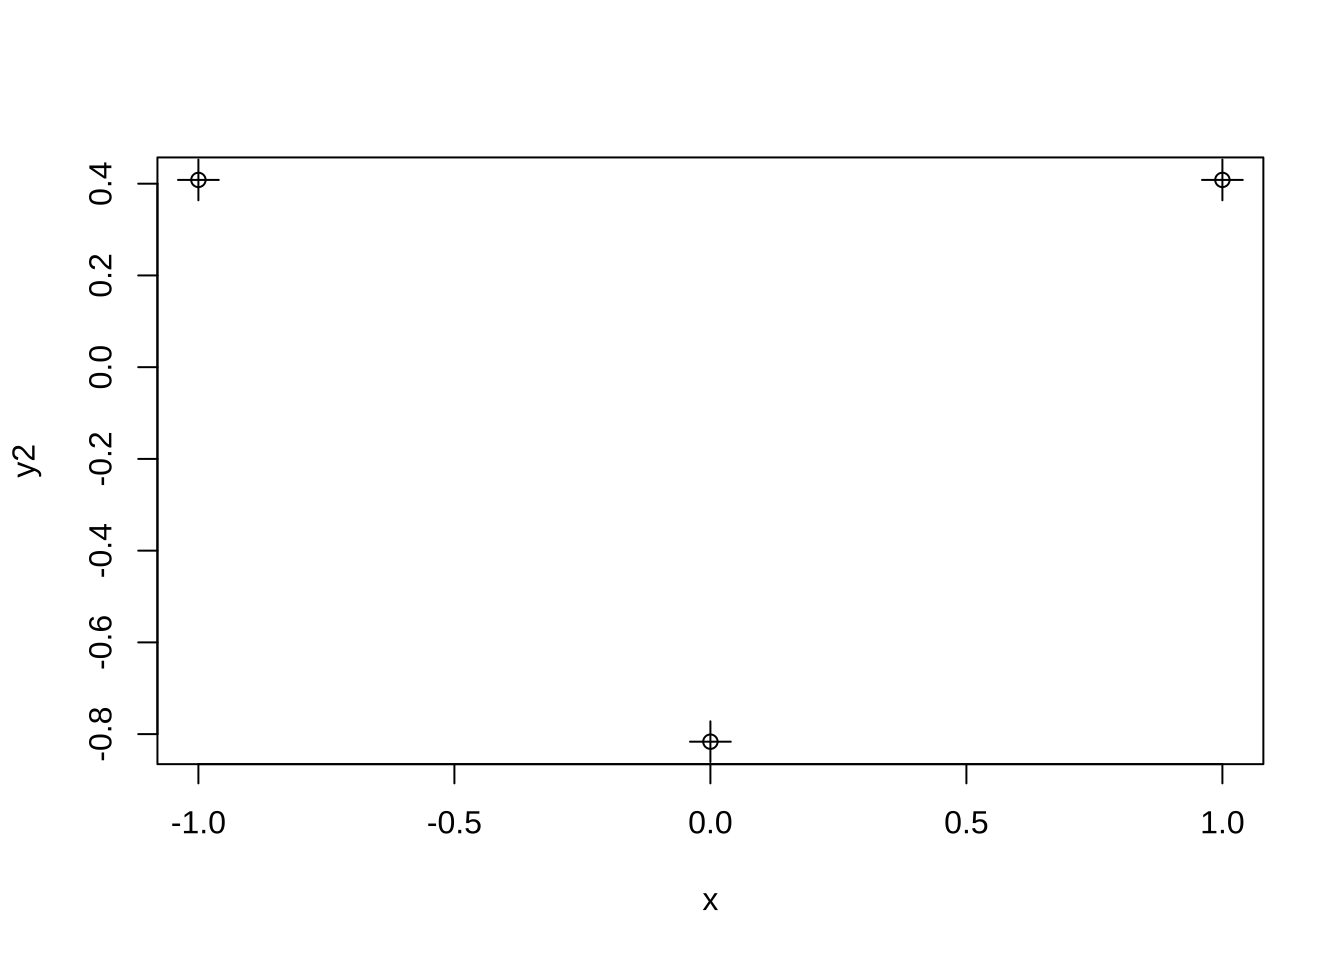
\includegraphics{hierarchical_files/figure-latex/unnamed-chunk-4-1.pdf}

예측된 각 개인의 절편과 기울기에 대한 임의효과의 예측값 \({\hat b}_{0i}\)과 \({\hat b}_{1i}\)에 고정효과의 추정량 \(\hat \beta_0\)와 \(\hat \beta_1\)에 각각 더해주면 각 개인의 절편과 기울기에 대한 예측값을 구할 수 있다.

\[ {\hat \beta}_{0i} = \hat \beta_0 + {\hat b}_{0i} , \quad 
{\hat \beta}_{1i} = \hat \beta_1 + {\hat b}_{1i} \]

\begin{Shaded}
\begin{Highlighting}[]
\NormalTok{beta }\OtherTok{\textless{}{-}} \FunctionTok{matrix}\NormalTok{(}\FunctionTok{as.numeric}\NormalTok{(}\FunctionTok{fixef}\NormalTok{(fm1)),}\DecValTok{18}\NormalTok{,}\DecValTok{2}\NormalTok{,}\AttributeTok{byrow=}\NormalTok{T)}
\NormalTok{beta }\SpecialCharTok{+}\NormalTok{ re }
\end{Highlighting}
\end{Shaded}

\begin{verbatim}
##     (Intercept)       Days
## 308    253.6637 19.6662617
## 309    211.0064  1.8476053
## 310    212.4447  5.0184295
## 330    275.0957  5.6529356
## 331    273.6654  7.3973743
## 332    260.4447 10.1951090
## 333    268.2456 10.2436499
## 334    244.1725 11.5418676
## 335    251.0714 -0.2848792
## 337    286.2956 19.0955511
## 349    226.1949 11.6407181
## 350    238.3351 17.0815038
## 351    255.9830  7.4520239
## 352    272.2688 14.0032871
## 369    254.6806 11.3395008
## 370    225.7921 15.2897709
## 371    252.2122  9.4791297
## 372    263.7197 11.7513080
\end{verbatim}

예를 들어 선형혼합모형에서 첫 번쨰 운전자에 대한 절편과 기울기에 대한 추정값은 다음과 같다.

\[ {\hat \beta}_{0i} =  253.6637,  \quad {\hat \beta}_{1i} = 19.6662617 \]

위의 결과를 각 운전자에 대해 개별 회귀직선 \eqref{eq:lmlist1}을 적합시켜서 얻은 18개의 절편과 기울기와 비교해보자.

\begin{Shaded}
\begin{Highlighting}[]
\FunctionTok{coef}\NormalTok{(lmf1)}
\end{Highlighting}
\end{Shaded}

\begin{verbatim}
##     (Intercept)      Days
## 308    244.1927 21.764702
## 309    205.0549  2.261785
## 310    203.4842  6.114899
## 330    289.6851  3.008073
## 331    285.7390  5.266019
## 332    264.2516  9.566768
## 333    275.0191  9.142045
## 334    240.1629 12.253141
## 335    263.0347 -2.881034
## 337    290.1041 19.025974
## 349    215.1118 13.493933
## 350    225.8346 19.504017
## 351    261.1470  6.433498
## 352    276.3721 13.566549
## 369    254.9681 11.348109
## 370    210.4491 18.056151
## 371    253.6360  9.188445
## 372    267.0448 11.298073
\end{verbatim}

이렇게 혼합모형을 통해서 얻은 각 개인의 절편과 기울기에 대한 예측값과 각각의 개인에 대해서 회귀직선을 따로 적합하여 얻은
절편과 기울기의 관계를 그림으로 그려보면 다음과 같다. 혼합모형을 통해서 얻은 각 개인의 절편과 기울기는 절편과 기울기의 전체평균값 방향으로 축소되는 경향(shrinkage)을 볼수있다.

\begin{Shaded}
\begin{Highlighting}[]
\NormalTok{df }\OtherTok{\textless{}{-}} \FunctionTok{coef}\NormalTok{(lmf1)}
\NormalTok{fclow }\OtherTok{\textless{}{-}} \FunctionTok{subset}\NormalTok{(df, }\StringTok{\textasciigrave{}}\AttributeTok{(Intercept)}\StringTok{\textasciigrave{}} \SpecialCharTok{\textless{}} \DecValTok{251}\NormalTok{)}
\NormalTok{fchigh }\OtherTok{\textless{}{-}} \FunctionTok{subset}\NormalTok{(df, }\StringTok{\textasciigrave{}}\AttributeTok{(Intercept)}\StringTok{\textasciigrave{}} \SpecialCharTok{\textgreater{}} \DecValTok{251}\NormalTok{)}
\NormalTok{cc1 }\OtherTok{\textless{}{-}} \FunctionTok{as.data.frame}\NormalTok{(}\FunctionTok{coef}\NormalTok{(fm1)}\SpecialCharTok{$}\NormalTok{Subject)}
\FunctionTok{names}\NormalTok{(cc1) }\OtherTok{\textless{}{-}} \FunctionTok{c}\NormalTok{(}\StringTok{"A"}\NormalTok{, }\StringTok{"B"}\NormalTok{)}
\NormalTok{df }\OtherTok{\textless{}{-}} \FunctionTok{cbind}\NormalTok{(df, cc1)}
\NormalTok{ff }\OtherTok{\textless{}{-}} \FunctionTok{fixef}\NormalTok{(fm1)}
\FunctionTok{with}\NormalTok{(df,}
     \FunctionTok{print}\NormalTok{(}\FunctionTok{xyplot}\NormalTok{(}\StringTok{\textasciigrave{}}\AttributeTok{(Intercept)}\StringTok{\textasciigrave{}} \SpecialCharTok{\textasciitilde{}}\NormalTok{ Days, }\AttributeTok{aspect =} \DecValTok{1}\NormalTok{,}
                  \AttributeTok{x1 =}\NormalTok{ B, }\AttributeTok{y1 =}\NormalTok{ A,}
                  \AttributeTok{panel =} \ControlFlowTok{function}\NormalTok{(x, y, x1, y1, subscripts, ...) \{}
                      \FunctionTok{panel.grid}\NormalTok{(}\AttributeTok{h =} \SpecialCharTok{{-}}\DecValTok{1}\NormalTok{, }\AttributeTok{v =} \SpecialCharTok{{-}}\DecValTok{1}\NormalTok{)}
\NormalTok{                      x1 }\OtherTok{\textless{}{-}}\NormalTok{ x1[subscripts]}
\NormalTok{                      y1 }\OtherTok{\textless{}{-}}\NormalTok{ y1[subscripts]}
                      \FunctionTok{larrows}\NormalTok{(x, y, x1, y1, }\AttributeTok{type =} \StringTok{"closed"}\NormalTok{, }\AttributeTok{length =} \FloatTok{0.1}\NormalTok{,}
                              \AttributeTok{angle =} \DecValTok{15}\NormalTok{, ...)}
                      \FunctionTok{lpoints}\NormalTok{(x, y,}
                              \AttributeTok{pch =} \FunctionTok{trellis.par.get}\NormalTok{(}\StringTok{"superpose.symbol"}\NormalTok{)}\SpecialCharTok{$}\NormalTok{pch[}\DecValTok{2}\NormalTok{],}
                              \AttributeTok{col =} \FunctionTok{trellis.par.get}\NormalTok{(}\StringTok{"superpose.symbol"}\NormalTok{)}\SpecialCharTok{$}\NormalTok{col[}\DecValTok{2}\NormalTok{])}
                      \FunctionTok{lpoints}\NormalTok{(x1, y1,}
                              \AttributeTok{pch =} \FunctionTok{trellis.par.get}\NormalTok{(}\StringTok{"superpose.symbol"}\NormalTok{)}\SpecialCharTok{$}\NormalTok{pch[}\DecValTok{1}\NormalTok{],}
                              \AttributeTok{col =} \FunctionTok{trellis.par.get}\NormalTok{(}\StringTok{"superpose.symbol"}\NormalTok{)}\SpecialCharTok{$}\NormalTok{col[}\DecValTok{1}\NormalTok{])}
                      \FunctionTok{lpoints}\NormalTok{(ff[}\DecValTok{2}\NormalTok{], ff[}\DecValTok{1}\NormalTok{], }
                              \AttributeTok{pch =} \FunctionTok{trellis.par.get}\NormalTok{(}\StringTok{"superpose.symbol"}\NormalTok{)}\SpecialCharTok{$}\NormalTok{pch[}\DecValTok{3}\NormalTok{],}
                              \AttributeTok{col =} \FunctionTok{trellis.par.get}\NormalTok{(}\StringTok{"superpose.symbol"}\NormalTok{)}\SpecialCharTok{$}\NormalTok{col[}\DecValTok{3}\NormalTok{])}
                      \FunctionTok{ltext}\NormalTok{(fclow[,}\DecValTok{2}\NormalTok{], fclow[,}\DecValTok{1}\NormalTok{], }\FunctionTok{row.names}\NormalTok{(fclow),}
                            \AttributeTok{adj =} \FunctionTok{c}\NormalTok{(}\FloatTok{0.5}\NormalTok{, }\FloatTok{1.7}\NormalTok{))}
                      \FunctionTok{ltext}\NormalTok{(fchigh[,}\DecValTok{2}\NormalTok{], fchigh[,}\DecValTok{1}\NormalTok{], }\FunctionTok{row.names}\NormalTok{(fchigh),}
                            \AttributeTok{adj =} \FunctionTok{c}\NormalTok{(}\FloatTok{0.5}\NormalTok{, }\SpecialCharTok{{-}}\FloatTok{0.6}\NormalTok{))}
\NormalTok{                  \},}
                  \AttributeTok{key =} \FunctionTok{list}\NormalTok{(}\AttributeTok{space =} \StringTok{"top"}\NormalTok{, }\AttributeTok{columns =} \DecValTok{3}\NormalTok{,}
                  \AttributeTok{text =} \FunctionTok{list}\NormalTok{(}\FunctionTok{c}\NormalTok{(}\StringTok{"Mixed model"}\NormalTok{, }\StringTok{"Individual"}\NormalTok{, }\StringTok{"Population"}\NormalTok{)),}
                   \AttributeTok{points =} \FunctionTok{list}\NormalTok{(}\AttributeTok{col =} \FunctionTok{trellis.par.get}\NormalTok{(}\StringTok{"superpose.symbol"}\NormalTok{)}\SpecialCharTok{$}\NormalTok{col[}\DecValTok{1}\SpecialCharTok{:}\DecValTok{3}\NormalTok{],}
                   \AttributeTok{pch =} \FunctionTok{trellis.par.get}\NormalTok{(}\StringTok{"superpose.symbol"}\NormalTok{)}\SpecialCharTok{$}\NormalTok{pch[}\DecValTok{1}\SpecialCharTok{:}\DecValTok{3}\NormalTok{]))}
\NormalTok{               )))}
\end{Highlighting}
\end{Shaded}

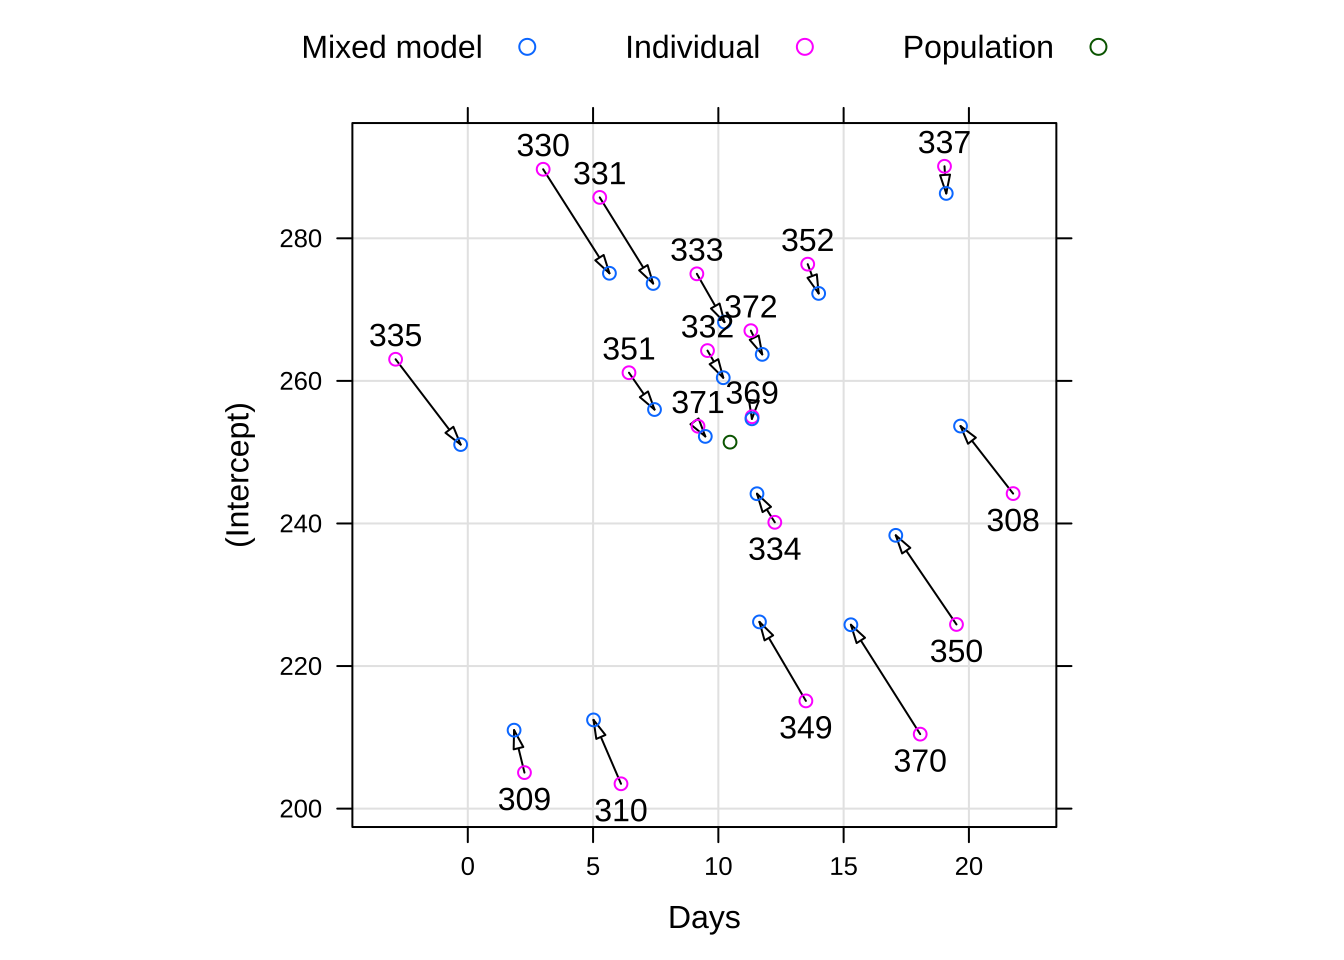
\includegraphics[width=.8\linewidth]{hierarchical_files/figure-latex/ex24 -1}

\hypertarget{uxbaa8uxd615uxc758-uxcd95uxc18c}{%
\subsection{모형의 축소}\label{uxbaa8uxd615uxc758-uxcd95uxc18c}}

위에서 고려한 임의계수모형 \eqref{eq:repeat}에서는 절편과 기울기에 대한 2개의 임의효과 \(b_{0i}\) 와 \(b_{1i}\) 를 고려하고 더 나아가 두 개의 임의효과가 독립이 아니며 상관계수가 \(\rho\)라고 가정하였다.

앞에서 추정결과에 의하면 두 개의 임의효과의 상관계수의 추정값은 \(\hat \rho = 0.066\) 으로 거의 0에 가깝다. 이러한 결과에 근거하여 두 임의효과가 독립인
축소모형을 고려해 보자. 즉 임의계수모형 \eqref{eq:repeat}에서 임의효과의 상관계수가 \(\rho=0\)인 임의효과의 분포를 다음과 같이 가정한다.

\[ 
\begin{bmatrix}
b_{0i} \\
b_{1i} \\
\end{bmatrix} \sim
N \left (
\begin{bmatrix}
0 \\
0 \\
\end{bmatrix}
,
\begin{bmatrix}
\sigma^2_{b1} & 0\\
0 & \sigma^2_{b2} \\
\end{bmatrix}
\right )
\]

이러한 모형을 아래와 같이 적합시키면 추정결과는 다음과 같다. 아래 모형식에서 \texttt{(1\ +\ Days\textbar{}\textbar{}Subject)}
는 각 개체 \texttt{Subject} 에 대하여 절편 \texttt{1} 과 기울기 \texttt{Days}에 임의효과를 포함한다고 지정하며 한개의 바 \texttt{\textbar{}} 대신 두 개의 바 \texttt{\textbar{}\textbar{}} 를 사용하면 임의효과가 독립이라는 것을 지정한다.

\begin{Shaded}
\begin{Highlighting}[]
\NormalTok{fm2 }\OtherTok{\textless{}{-}} \FunctionTok{lmer}\NormalTok{(Reaction }\SpecialCharTok{\textasciitilde{}} \DecValTok{1} \SpecialCharTok{+}\NormalTok{ Days }\SpecialCharTok{+}\NormalTok{ (}\DecValTok{1}\SpecialCharTok{+}\NormalTok{Days }\SpecialCharTok{||}\NormalTok{ Subject) , sleepstudy)}
\FunctionTok{summary}\NormalTok{(fm2)}
\end{Highlighting}
\end{Shaded}

\begin{verbatim}
## Linear mixed model fit by REML. t-tests use Satterthwaite's method [
## lmerModLmerTest]
## Formula: Reaction ~ 1 + Days + (1 + Days || Subject)
##    Data: sleepstudy
## 
## REML criterion at convergence: 1743.7
## 
## Scaled residuals: 
##     Min      1Q  Median      3Q     Max 
## -3.9626 -0.4625  0.0204  0.4653  5.1860 
## 
## Random effects:
##  Groups    Name        Variance Std.Dev.
##  Subject   (Intercept) 627.57   25.051  
##  Subject.1 Days         35.86    5.988  
##  Residual              653.58   25.565  
## Number of obs: 180, groups:  Subject, 18
## 
## Fixed effects:
##             Estimate Std. Error      df t value Pr(>|t|)    
## (Intercept)  251.405      6.885  18.156  36.513  < 2e-16 ***
## Days          10.467      1.560  18.156   6.712 2.59e-06 ***
## ---
## Signif. codes:  0 '***' 0.001 '**' 0.01 '*' 0.05 '.' 0.1 ' ' 1
## 
## Correlation of Fixed Effects:
##      (Intr)
## Days -0.184
\end{verbatim}

상관계수가 0인 모형에 대한 추정 결과는 상관계수가 있는 모형과 크게 다르지 않다.

두 모형, 즉 절편과 기울기에 대한 두 임의효과가 종속인지 또는 독립인지에 대한 두 모형을 AIC(Akaike Information Criteris)와 BIC(Bayesian Information Criteria)로 비교한 결과이다. 두 모형 간의 차이는 거의 없는 것으로 판단된다.

\begin{Shaded}
\begin{Highlighting}[]
\FunctionTok{c}\NormalTok{(}\FunctionTok{AIC}\NormalTok{(fm1) , }\FunctionTok{BIC}\NormalTok{(fm1))}
\end{Highlighting}
\end{Shaded}

\begin{verbatim}
## [1] 1755.628 1774.786
\end{verbatim}

\begin{Shaded}
\begin{Highlighting}[]
\FunctionTok{c}\NormalTok{(}\FunctionTok{AIC}\NormalTok{(fm2), }\FunctionTok{BIC}\NormalTok{(fm2))}
\end{Highlighting}
\end{Shaded}

\begin{verbatim}
## [1] 1753.669 1769.634
\end{verbatim}

더나아가 \texttt{anova} 함수를 이용하여 두 모형의 차이를 검정한 결과는 두 모형 간의 차이가 없다는 것이다. 참고할 점은 혼합모형에서의 모형을 비교하는 분산분석에 의한 검정은 효율이 떨어질 수 있기 때문에 주의해야 한다.

\begin{Shaded}
\begin{Highlighting}[]
\FunctionTok{anova}\NormalTok{(fm1,fm2)}
\end{Highlighting}
\end{Shaded}

\begin{verbatim}
## refitting model(s) with ML (instead of REML)
\end{verbatim}

\begin{verbatim}
## Data: sleepstudy
## Models:
## fm2: Reaction ~ 1 + Days + (1 + Days || Subject)
## fm1: Reaction ~ 1 + Days + (1 + Days | Subject)
##     npar    AIC    BIC  logLik deviance  Chisq Df Pr(>Chisq)
## fm2    5 1762.0 1778.0 -876.00   1752.0                     
## fm1    6 1763.9 1783.1 -875.97   1751.9 0.0639  1     0.8004
\end{verbatim}

\hypertarget{uxbca0uxc774uxc9c0uxc548-uxcd94uxc815}{%
\section{베이지안 추정}\label{uxbca0uxc774uxc9c0uxc548-uxcd94uxc815}}

임의효과를 이용하는 선형혼합 모형은 모형의 구조상 베이지안 모형과 매우 유사하다. 베이지안 모형에서는 회귀계수와 분산 성분에 대한 사전분포(prior distribution)을 설정하고 모수들의 사후분포(posterior distribution)을 추정한다.

베이지안 모형의 적합은 매우 다양한 패키지나 프로그램을 사용할 수 있다(\texttt{BUGS},\texttt{STAN}, \texttt{MCMCglmm}, \texttt{brms}). 본 강의에서는 \texttt{brms} 패키지의 \texttt{brm} 함수를 사용하여 베이지안 방법으로 임의계수 모형을 적합하는 예를 보여주고자 한다. \texttt{brms} 패키지는 \texttt{lme4} 패키지의 모형식을 그대로 사용할 수 있다. 참고로 다른 패키지는 \texttt{lme4} 패키지의 모형식보다 더욱 복잡한 식을 사용해야 한다.

\texttt{sleepstudy} 자료에 대하여 \texttt{brms} 패키지의 \texttt{brm} 함수를 이용하여 베이지안 방법으로 임의계수 모형을 추정하는 프로그램은 아래와 같다.

\begin{Shaded}
\begin{Highlighting}[]
\NormalTok{fm3 }\OtherTok{\textless{}{-}} \FunctionTok{brm}\NormalTok{(Reaction }\SpecialCharTok{\textasciitilde{}} \DecValTok{1} \SpecialCharTok{+}\NormalTok{ Days }\SpecialCharTok{+}\NormalTok{ (}\DecValTok{1} \SpecialCharTok{+}\NormalTok{ Days}\SpecialCharTok{|}\NormalTok{Subject), }\AttributeTok{data =}\NormalTok{ sleepstudy)}
\end{Highlighting}
\end{Shaded}

\begin{verbatim}
## Compiling Stan program...
\end{verbatim}

\begin{verbatim}
## Start sampling
\end{verbatim}

\begin{verbatim}
## 
## SAMPLING FOR MODEL '9911b459d8c4b04b2868a198ead77672' NOW (CHAIN 1).
## Chain 1: 
## Chain 1: Gradient evaluation took 7.2e-05 seconds
## Chain 1: 1000 transitions using 10 leapfrog steps per transition would take 0.72 seconds.
## Chain 1: Adjust your expectations accordingly!
## Chain 1: 
## Chain 1: 
## Chain 1: Iteration:    1 / 2000 [  0%]  (Warmup)
## Chain 1: Iteration:  200 / 2000 [ 10%]  (Warmup)
## Chain 1: Iteration:  400 / 2000 [ 20%]  (Warmup)
## Chain 1: Iteration:  600 / 2000 [ 30%]  (Warmup)
## Chain 1: Iteration:  800 / 2000 [ 40%]  (Warmup)
## Chain 1: Iteration: 1000 / 2000 [ 50%]  (Warmup)
## Chain 1: Iteration: 1001 / 2000 [ 50%]  (Sampling)
## Chain 1: Iteration: 1200 / 2000 [ 60%]  (Sampling)
## Chain 1: Iteration: 1400 / 2000 [ 70%]  (Sampling)
## Chain 1: Iteration: 1600 / 2000 [ 80%]  (Sampling)
## Chain 1: Iteration: 1800 / 2000 [ 90%]  (Sampling)
## Chain 1: Iteration: 2000 / 2000 [100%]  (Sampling)
## Chain 1: 
## Chain 1:  Elapsed Time: 1.61174 seconds (Warm-up)
## Chain 1:                0.570718 seconds (Sampling)
## Chain 1:                2.18246 seconds (Total)
## Chain 1: 
## 
## SAMPLING FOR MODEL '9911b459d8c4b04b2868a198ead77672' NOW (CHAIN 2).
## Chain 2: 
## Chain 2: Gradient evaluation took 2.4e-05 seconds
## Chain 2: 1000 transitions using 10 leapfrog steps per transition would take 0.24 seconds.
## Chain 2: Adjust your expectations accordingly!
## Chain 2: 
## Chain 2: 
## Chain 2: Iteration:    1 / 2000 [  0%]  (Warmup)
## Chain 2: Iteration:  200 / 2000 [ 10%]  (Warmup)
## Chain 2: Iteration:  400 / 2000 [ 20%]  (Warmup)
## Chain 2: Iteration:  600 / 2000 [ 30%]  (Warmup)
## Chain 2: Iteration:  800 / 2000 [ 40%]  (Warmup)
## Chain 2: Iteration: 1000 / 2000 [ 50%]  (Warmup)
## Chain 2: Iteration: 1001 / 2000 [ 50%]  (Sampling)
## Chain 2: Iteration: 1200 / 2000 [ 60%]  (Sampling)
## Chain 2: Iteration: 1400 / 2000 [ 70%]  (Sampling)
## Chain 2: Iteration: 1600 / 2000 [ 80%]  (Sampling)
## Chain 2: Iteration: 1800 / 2000 [ 90%]  (Sampling)
## Chain 2: Iteration: 2000 / 2000 [100%]  (Sampling)
## Chain 2: 
## Chain 2:  Elapsed Time: 1.03919 seconds (Warm-up)
## Chain 2:                0.648274 seconds (Sampling)
## Chain 2:                1.68746 seconds (Total)
## Chain 2: 
## 
## SAMPLING FOR MODEL '9911b459d8c4b04b2868a198ead77672' NOW (CHAIN 3).
## Chain 3: 
## Chain 3: Gradient evaluation took 2.2e-05 seconds
## Chain 3: 1000 transitions using 10 leapfrog steps per transition would take 0.22 seconds.
## Chain 3: Adjust your expectations accordingly!
## Chain 3: 
## Chain 3: 
## Chain 3: Iteration:    1 / 2000 [  0%]  (Warmup)
## Chain 3: Iteration:  200 / 2000 [ 10%]  (Warmup)
## Chain 3: Iteration:  400 / 2000 [ 20%]  (Warmup)
## Chain 3: Iteration:  600 / 2000 [ 30%]  (Warmup)
## Chain 3: Iteration:  800 / 2000 [ 40%]  (Warmup)
## Chain 3: Iteration: 1000 / 2000 [ 50%]  (Warmup)
## Chain 3: Iteration: 1001 / 2000 [ 50%]  (Sampling)
## Chain 3: Iteration: 1200 / 2000 [ 60%]  (Sampling)
## Chain 3: Iteration: 1400 / 2000 [ 70%]  (Sampling)
## Chain 3: Iteration: 1600 / 2000 [ 80%]  (Sampling)
## Chain 3: Iteration: 1800 / 2000 [ 90%]  (Sampling)
## Chain 3: Iteration: 2000 / 2000 [100%]  (Sampling)
## Chain 3: 
## Chain 3:  Elapsed Time: 1.1138 seconds (Warm-up)
## Chain 3:                0.518563 seconds (Sampling)
## Chain 3:                1.63236 seconds (Total)
## Chain 3: 
## 
## SAMPLING FOR MODEL '9911b459d8c4b04b2868a198ead77672' NOW (CHAIN 4).
## Chain 4: 
## Chain 4: Gradient evaluation took 2.2e-05 seconds
## Chain 4: 1000 transitions using 10 leapfrog steps per transition would take 0.22 seconds.
## Chain 4: Adjust your expectations accordingly!
## Chain 4: 
## Chain 4: 
## Chain 4: Iteration:    1 / 2000 [  0%]  (Warmup)
## Chain 4: Iteration:  200 / 2000 [ 10%]  (Warmup)
## Chain 4: Iteration:  400 / 2000 [ 20%]  (Warmup)
## Chain 4: Iteration:  600 / 2000 [ 30%]  (Warmup)
## Chain 4: Iteration:  800 / 2000 [ 40%]  (Warmup)
## Chain 4: Iteration: 1000 / 2000 [ 50%]  (Warmup)
## Chain 4: Iteration: 1001 / 2000 [ 50%]  (Sampling)
## Chain 4: Iteration: 1200 / 2000 [ 60%]  (Sampling)
## Chain 4: Iteration: 1400 / 2000 [ 70%]  (Sampling)
## Chain 4: Iteration: 1600 / 2000 [ 80%]  (Sampling)
## Chain 4: Iteration: 1800 / 2000 [ 90%]  (Sampling)
## Chain 4: Iteration: 2000 / 2000 [100%]  (Sampling)
## Chain 4: 
## Chain 4:  Elapsed Time: 1.0575 seconds (Warm-up)
## Chain 4:                0.581012 seconds (Sampling)
## Chain 4:                1.63851 seconds (Total)
## Chain 4:
\end{verbatim}

\begin{Shaded}
\begin{Highlighting}[]
\NormalTok{fm3}
\end{Highlighting}
\end{Shaded}

\begin{verbatim}
##  Family: gaussian 
##   Links: mu = identity; sigma = identity 
## Formula: Reaction ~ 1 + Days + (1 + Days | Subject) 
##    Data: sleepstudy (Number of observations: 180) 
## Samples: 4 chains, each with iter = 2000; warmup = 1000; thin = 1;
##          total post-warmup samples = 4000
## 
## Group-Level Effects: 
## ~Subject (Number of levels: 18) 
##                     Estimate Est.Error l-95% CI u-95% CI Rhat Bulk_ESS Tail_ESS
## sd(Intercept)          27.12      6.95    15.53    42.53 1.00     1761     2389
## sd(Days)                6.66      1.61     4.21    10.31 1.00     1289     1359
## cor(Intercept,Days)     0.09      0.30    -0.47     0.69 1.00      927     1540
## 
## Population-Level Effects: 
##           Estimate Est.Error l-95% CI u-95% CI Rhat Bulk_ESS Tail_ESS
## Intercept   251.47      7.59   236.47   266.10 1.00     1668     2446
## Days         10.41      1.76     7.01    13.88 1.00     1173     1341
## 
## Family Specific Parameters: 
##       Estimate Est.Error l-95% CI u-95% CI Rhat Bulk_ESS Tail_ESS
## sigma    25.85      1.53    23.06    29.07 1.00     2827     2619
## 
## Samples were drawn using sampling(NUTS). For each parameter, Bulk_ESS
## and Tail_ESS are effective sample size measures, and Rhat is the potential
## scale reduction factor on split chains (at convergence, Rhat = 1).
\end{verbatim}

\hypertarget{sae}{%
\chapter{소지역추정}\label{sae}}

층화추출을 이용하는 표본조사(stratified sampling)에서 층에 배정된 표본수가 적을 경우에는 특성이 유사한 인근의 층의 추출단위들을 결합하여 추출단위들의 그룹을 만들고 그 그룹 내에서 추출단위들은 동일한 특성을 갖는다고 가정할 수 있으면 유사한 인근의 조사결과를 활용해서 좀더 정도높은 추정값을 작성할 수 있다.

이와 같이 비슷한 특성을 갖는 인근의 조사결과나 행정업무자료 또는 센서스 등 다른 통계조사 정보를 조사된 자료에서 얻은 직접 추정값과 결합하여 세부단위에 대한 통계를 작성하는 기법을 \textbf{소지역 추정법(Small Area Estimation)}이라고 한다.

소지역 추정법은 지역 수준모형(area-level model)과 단위 수준모형(unit-level model)이 있다.

\begin{itemize}
\tightlist
\item
  지역 수준모형: 지역과 관련된 직접추정량과 지역의 보조자료를 결합한 모형
\item
  단위 수준모형: 지역과 관련된 직접추정량과 지역 안의 추출단위에 대한 보조자료를 결합한 모형
\end{itemize}

이 강의 예제에서는 단위 수준모형만 다룰 것이다.

\hypertarget{uxb2e8uxc704-uxc218uxc900uxbaa8uxd615uxc758-uxac1cuxc694}{%
\section{단위 수준모형의 개요}\label{uxb2e8uxc704-uxc218uxc900uxbaa8uxd615uxc758-uxac1cuxc694}}

\hypertarget{uxbaa8uxc9d1uxb2e8uxc5d0-uxb300uxd55c-uxac00uxc815}{%
\subsection{모집단에 대한 가정}\label{uxbaa8uxc9d1uxb2e8uxc5d0-uxb300uxd55c-uxac00uxc815}}

모집딘 \(U\) 가 \(D\) 개의 층으로 나누어져 있다고 가정하자, 층 \(U_1, U_2, \dots, U_D\)는
서로 겹치지 않는 작은 세부단위이며 각 층에는 각각 \(N_1, N_2, \dots, N_D\)의 추출단위가 있다고 하자.

이제 \(Y_{dj}\) 를 층 \(d\)에 속하는 \(i\) 번째 단위가 가진 값이라고 하자. 층 \(d\)에 속하는 모든 반응값들을 벡터로 표시하면 \(\bm y_d = (Y_{d1}, Y_{d2}, \cdots, Y_{dN_{d}})^t\) 이다.

이제 추정하고 싶은 모수는 층별 모평균 \(\bar Y_d\) 이다.

\[ \bar Y_d = \frac{ \sum_{j=1}^{N_s} Y_{dj} } { N_d} \]

이제 층별 모평균을 추정하기 위하여 층 \(U_d\) 에서 \(n_d\) 개의 표본 \(s_d\)를 추츨한다.
총 표본의 수 \(n= \sum_d n_d\) 는 각 층에서 추출한 표본의 수의 합니다.

소지역에서 표본에 속하지 않는 단위들의 집합을 \(r_d\)로 표기한다.

\hypertarget{uxbcf4uxc870-uxc815uxbcf4uxc640-uxacc4uxce35-uxbaa8uxd615}{%
\subsection{보조 정보와 계층 모형}\label{uxbcf4uxc870-uxc815uxbcf4uxc640-uxacc4uxce35-uxbaa8uxd615}}

이제 추출 단위(sampling unit)에 대한 보보 정보가 있다고 하자.
보조 정보는 추출 단위들의 실제값 \(y_{dj}\) 에 대한 정보를 지니고 있으며 \(p\)개의 변수로 구성되어 있다고 가정하자.

추출 단위에 대한 보조 정보 \(\bm x_{dj}\) 는 추출단위의 관심 변수 \(Y_{dj}\) 와 다음과 같은 계층보형의 관계를 가진다고 가정한다.
이러한 모형은 \citep{battese1988error}에 의하여 제안된 선형 혼합효과 모형이다.

\begin{equation}
Y_{dj} = {\bm x}_{dj}^t \bm \beta + u_d + e_{dj}
\label{eq:bhfmodel}
\end{equation}

위 식 \eqref{eq:bhfmodel} 에서 \(u_d\)는 임의효과로서 소지역 \(U_d\)에 대한 효과(area effect)를 반영한다. 또한 \(e_{dj}\) 는 추출단의의 오차이다. 소지역 효과 \(u_d\)와 오차항 \(e_{dj}\) 는 다음과 같이 각각 정규분포를 따른다.

\begin{equation}
u_d \sim N(0, \sigma^2_u), \quad e_{dj} \sim N(0, \sigma^2_e)
\label{eq:dist}
\end{equation}

소지역 효과 \(u_d\)와 오차항 \(e_{dj}\) 는 서로 독립이며
분산성분 \(\sigma^2_u\) 과 \(\sigma^2_e\)는 모르는 모수로 추정을 해야한다.

\hypertarget{uxcd94uxc815uxbc95}{%
\subsection{추정법}\label{uxcd94uxc815uxbc95}}

단위 수준모형 \eqref{eq:bhfmodel}에서 소지역 평균 \(\bar Y_d\)에 대한 추정량은
다음과 같은 최적 선형불편 예측량(Best Linear Unbiased Prediction; BLUP)으로 주어진다.
\citep{royall1970finite}.

\begin{equation}
\tilde {\bar Y}_d^{BLUP}  = \frac{1}{N_d} \left  [ \sum_{j \in s_d} Y_{dj} 
+ \sum_{j \in r_d} \tilde Y_{dj} \right ] 
\label{eq:blup1}
\end{equation}

추정식 \eqref{eq:blup1} 에서 표본에 속하지 않은 단위들에 대한 추정량 \(\tilde Y_{dj}\) 은 다음과 같이 주어진다.

\[ \tilde Y_{dj} = {\bm x}_{dj}^t \tilde {\bm \beta} + \tilde u_d \]
위의 식에서 \(\tilde u_d\) 는 소지역의 임의효과 \(u_d\) 에 대한 최적 선형불편 예측량(BLUP)이며 다음과 같이 표시할 수 있다.

\[ \tilde u_d = \gamma_d ( \bar y_{ds} - \bar { \bm x}_{ds}^t  \tilde {\bm \beta} ) \]
여기서

\begin{itemize}
\item
  \(\bar y_{ds}= \sum_{j \in s_d} Y_{dj}/ n_d\) 는 소지역 \(d\) 에서 추출된 관심변수 표본의 평균
\item
  \(\bar {\bm x}_{ds}= \sum_{j \in s_d} {\bm x}_{dj}/ n_d\) 는 소지역 \(d\) 에서 추출된 보조변수 표본의 평균
\end{itemize}

또한 같은 소지역에 소과는 단위들의 상관관계를 의미하는 \(\gamma_d\)는 다음과 같다.

\[ \gamma_d = \frac{ \sigma_u^2}{\sigma_u^2 + \sigma_e^2 / n_d}\]

위의 추정식들에서 분산성분 \(\sigma^2_u\) 과 \(\sigma^2_e\)은 모르는 모수이므로
최대가능도 추정(또는 제한적 최대 가능도 추정량, REML)을 통하여 추정하여야 한다.

추정된 분산성분을 다시 추정식 @res(eq:blup1) 에 대입하고 최종적으로 정리하면 소지역 추정량은 다음과 같이 주어진다.

\begin{equation}
\hat {\bar Y}_d^{BLUP} = f_d \bar y_{ds} + (\bar {\bm X}_d - f_d \bar {\bm x}_{ds})^t
\hat {\bm \beta} + (1-f_d) \hat u_d 
\label{eq:blup2}
\end{equation}

여기서 \(f_d = n_d/N_d\) 로서 표본 비율이다. 최종 소지역 추정식 @res(eq:blup2) 를 보면
보조 변수의 모집단 평균 \(\bar {\bm X}_d\)rk 필요한 것을 알 수 있다.

위의 소지역 추정에 대한 요약은 \citep{molina2015sae}에 더 자세한 내용이 있다.

\hypertarget{uxc608uxc81c}{%
\section{예제}\label{uxc608uxc81c}}

예제에서는 자영업이 많은 부분을 차지하고 있는 음식점에 대한 경제자료를 이용하여 표본 평균을 이용한 단순추정량과 소지역 모형을 사용한 추정량을 비교하려고 한다.

분석 자료는 A지역의 사업체를 한식음식점을 대상으로 제한하여 사용하였다.

\begin{itemize}
\item
  표본설계는 동(소지역)을 층으로 하는 단순층화추출을 사용하였다.
\item
  관심변수는 매출액을 고려하였다.
\item
  2개의 보조변수는 재료구입비와 연간급여액을 고려하였다. 연간급여액과 재료구입비는 고용 보험 및 신용카드 내역을 통해 모든 사업체에 대해여 얻을 수 있는 자료로 지역 추정 모형에서 보조변수로 활용하였다.
\end{itemize}

두 보조자료를 바탕으로 매출액을 추정하는 소지역 추정 모형을 세워 단순 추정과 비교하고자 한다. 분석 자료에서 쓰이는 변수의 단위는 모두 `백만원'이다.

분석에 사용되는 모집단 자료의 개수는 총 10167 개로 A지역은 총 326개의 동(소지역, 층)로 나뉜다.

모의실험에서 표본 자료는 1489 개의 음식점을 추출하여 사용하였으며, 이를 추출하기 위하여 모집단의 각 동의 수에 비례하는 층화추출 방법을 사용하였다.

분석에서 사용되는 변수와 의미는 다음과 같다.

\begin{itemize}
\tightlist
\item
  \texttt{SLE\_ALL\_AMT"}: 매출액
\item
  \texttt{MNF\_PCST} :재료구입비
\item
  \texttt{SURV\_PHS\_SLR\_SUM} : 연간급여액
\item
  \texttt{AD\_CD} : 지역코드
\end{itemize}

\hypertarget{uxc790uxb8cc-uxc785uxb825-uxbc0f-uxc815uxb9ac}{%
\subsection{자료 입력 및 정리}\label{uxc790uxb8cc-uxc785uxb825-uxbc0f-uxc815uxb9ac}}

\begin{Shaded}
\begin{Highlighting}[]
\CommentTok{\# SEED 고정}
\FunctionTok{set.seed}\NormalTok{(}\DecValTok{321}\NormalTok{)  }

\CommentTok{\# 자료읽기}
\NormalTok{data }\OtherTok{\textless{}{-}} \FunctionTok{read.sas7bdat}\NormalTok{(}\StringTok{"/Users/ylee19067/Dropbox/working/teaching/kimhj/sas/derived/fin\_data.sas7bdat"}\NormalTok{)}

\CommentTok{\# 필요한 변수 선택 }
\NormalTok{data }\OtherTok{\textless{}{-}}\NormalTok{ data[}\FunctionTok{c}\NormalTok{(}\StringTok{"SURV\_PHS\_SLR\_SUM"}\NormalTok{, }\StringTok{"SLE\_ALL\_AMT"}\NormalTok{, }\StringTok{"MNF\_PCST"}\NormalTok{ , }\StringTok{"AD\_CD"}\NormalTok{)]}

\CommentTok{\# 자료를 지역번호 순으로 정렬 }
\NormalTok{data }\OtherTok{\textless{}{-}}\NormalTok{ data[}\FunctionTok{order}\NormalTok{(data}\SpecialCharTok{$}\NormalTok{AD\_CD), ]}

\CommentTok{\# 지역코드를 범주화 변수로 변환}
\NormalTok{data}\SpecialCharTok{$}\NormalTok{AD\_CD }\OtherTok{\textless{}{-}} \FunctionTok{as.factor}\NormalTok{(data}\SpecialCharTok{$}\NormalTok{AD\_CD)}

\FunctionTok{head}\NormalTok{(data, }\AttributeTok{n=}\DecValTok{10}\NormalTok{)}
\end{Highlighting}
\end{Shaded}

\begin{verbatim}
##      SURV_PHS_SLR_SUM SLE_ALL_AMT MNF_PCST   AD_CD
## 42                 14         103       23 1101053
## 44                 13          40       16 1101053
## 45                  4          40       15 1101053
## 878                12         100       38 1101053
## 901                 2          20        8 1101053
## 909                 7          36       14 1101053
## 910                 1          30        9 1101053
## 920                 7          15        6 1101053
## 921                 2          15        6 1101053
## 1028                5          56       15 1101053
\end{verbatim}

\hypertarget{uxbaa8uxc9d1uxb2e8-uxc815uxbcf4-uxc0dduxc131}{%
\subsection{모집단 정보 생성}\label{uxbaa8uxc9d1uxb2e8-uxc815uxbcf4-uxc0dduxc131}}

\begin{Shaded}
\begin{Highlighting}[]
\CommentTok{\# 모집단에서 각 동에 속한 사업체의 수를 계산  }
\NormalTok{gu }\OtherTok{\textless{}{-}}  \FunctionTok{unique}\NormalTok{(data}\SpecialCharTok{$}\NormalTok{AD\_CD)}
\NormalTok{gugu }\OtherTok{\textless{}{-}} \FunctionTok{table}\NormalTok{(data}\SpecialCharTok{$}\NormalTok{AD\_CD)}
\FunctionTok{head}\NormalTok{(gugu, }\AttributeTok{n=}\DecValTok{20}\NormalTok{)}
\end{Highlighting}
\end{Shaded}

\begin{verbatim}
## 
## 1101053 1101054 1101055 1101056 1101057 1101058 1101060 1101061 1101063 1101064 
##     111      23       7      22       3      11      33     274      60      37 
## 1101065 1101066 1101067 1101068 1101069 1101070 1101071 1101072 1102052 1102054 
##      38       4      21      14       4      14      18      16     125      85
\end{verbatim}

\hypertarget{uxc0acuxc5c5uxccb4uxc758-uxc218uxac00-10uxac1c-uxbbf8uxb9ccuxc778-uxb3d9uxc744-uxc81cuxac70}{%
\subsection{사업체의 수가 10개 미만인 동을 제거}\label{uxc0acuxc5c5uxccb4uxc758-uxc218uxac00-10uxac1c-uxbbf8uxb9ccuxc778-uxb3d9uxc744-uxc81cuxac70}}

표본 추출할 경우 사업체으 수가 극단적으로 작은 동은 표본의 배정이 사업체의 수보다 많아질 수 있으므로
사업체의 수가 10 미만인 동을 모집단에서 제거한다.

\begin{Shaded}
\begin{Highlighting}[]
\CommentTok{\# 사업체의 수가 10 미만인 동을 제거}
\NormalTok{smalldong }\OtherTok{\textless{}{-}} \FunctionTok{names}\NormalTok{(gugu[gugu }\SpecialCharTok{\textless{}} \DecValTok{10}\NormalTok{])}
\NormalTok{data }\OtherTok{\textless{}{-}}\NormalTok{ data }\SpecialCharTok{\%\textgreater{}\%} \FunctionTok{rowwise}\NormalTok{() }\SpecialCharTok{\%\textgreater{}\%} \FunctionTok{filter}\NormalTok{(}\SpecialCharTok{!}\NormalTok{AD\_CD }\SpecialCharTok{\%in\%}\NormalTok{ smalldong) }
\NormalTok{data}\SpecialCharTok{$}\NormalTok{AD\_CD }\OtherTok{\textless{}{-}} \FunctionTok{droplevels}\NormalTok{(data}\SpecialCharTok{$}\NormalTok{AD\_CD)}
\CommentTok{\# 모집단에서 각 동에 속한 사업체의 수를 다시 계산  }
\NormalTok{gugu }\OtherTok{=} \FunctionTok{table}\NormalTok{(data}\SpecialCharTok{$}\NormalTok{AD\_CD)}
\FunctionTok{head}\NormalTok{(gugu, }\AttributeTok{n=}\DecValTok{20}\NormalTok{)}
\end{Highlighting}
\end{Shaded}

\begin{verbatim}
## 
## 1101053 1101054 1101056 1101058 1101060 1101061 1101063 1101064 1101065 1101067 
##     111      23      22      11      33     274      60      37      38      21 
## 1101068 1101070 1101071 1101072 1102052 1102054 1102055 1102057 1102058 1102059 
##      14      14      18      16     125      85     188      41      24      61
\end{verbatim}

\hypertarget{uxcd5cuxc885-uxbaa8uxc9d1uxb2e8uxc758-uxc218}{%
\subsection{최종 모집단의 수}\label{uxcd5cuxc885-uxbaa8uxc9d1uxb2e8uxc758-uxc218}}

\begin{Shaded}
\begin{Highlighting}[]
\FunctionTok{dim}\NormalTok{(data)}
\end{Highlighting}
\end{Shaded}

\begin{verbatim}
## [1] 10167     4
\end{verbatim}

\begin{itemize}
\item
  최종 모집단에서 음식점의 수는 10167 개이다.
\item
  최종 모집단에서 소지역(동)의 개수는 326 개이다.
\end{itemize}

\hypertarget{uxad00uxc2ecuxbcc0uxc218uxc640-uxbcf4uxc870uxbcc0uxc218uxc758-uxad00uxacc4}{%
\subsection{관심변수와 보조변수의 관계}\label{uxad00uxc2ecuxbcc0uxc218uxc640-uxbcf4uxc870uxbcc0uxc218uxc758-uxad00uxacc4}}

이제 모집단에서 매출액과 재료 구입비에 대한 관계를 회귀분석으로 분석해 보자.

\begin{Shaded}
\begin{Highlighting}[]
\NormalTok{line1 }\OtherTok{\textless{}{-}} \FunctionTok{lm}\NormalTok{(data}\SpecialCharTok{$}\NormalTok{SLE\_ALL\_AMT }\SpecialCharTok{\textasciitilde{}}\NormalTok{ data}\SpecialCharTok{$}\NormalTok{MNF\_PCST)}
\FunctionTok{summary}\NormalTok{(line1)}
\end{Highlighting}
\end{Shaded}

\begin{verbatim}
## 
## Call:
## lm(formula = data$SLE_ALL_AMT ~ data$MNF_PCST)
## 
## Residuals:
##     Min      1Q  Median      3Q     Max 
## -3759.3   -52.0   -25.8    20.7  8228.3 
## 
## Coefficients:
##               Estimate Std. Error t value Pr(>|t|)    
## (Intercept)   58.92009    2.66787   22.09   <2e-16 ***
## data$MNF_PCST  2.01593    0.01018  197.94   <2e-16 ***
## ---
## Signif. codes:  0 '***' 0.001 '**' 0.01 '*' 0.05 '.' 0.1 ' ' 1
## 
## Residual standard error: 230.2 on 10165 degrees of freedom
## Multiple R-squared:  0.794,  Adjusted R-squared:  0.794 
## F-statistic: 3.918e+04 on 1 and 10165 DF,  p-value: < 2.2e-16
\end{verbatim}

\begin{Shaded}
\begin{Highlighting}[]
\FunctionTok{plot}\NormalTok{(data}\SpecialCharTok{$}\NormalTok{SLE\_ALL\_AMT }\SpecialCharTok{\textasciitilde{}}\NormalTok{ data}\SpecialCharTok{$}\NormalTok{MNF\_PCST, }\AttributeTok{xlab=}\StringTok{\textquotesingle{}재료구입비\textquotesingle{}}\NormalTok{, }\AttributeTok{ylab=}\StringTok{\textquotesingle{}매출액\textquotesingle{}}\NormalTok{)}
\FunctionTok{abline}\NormalTok{(line1, }\AttributeTok{col=}\StringTok{\textquotesingle{}red\textquotesingle{}}\NormalTok{)}
\end{Highlighting}
\end{Shaded}

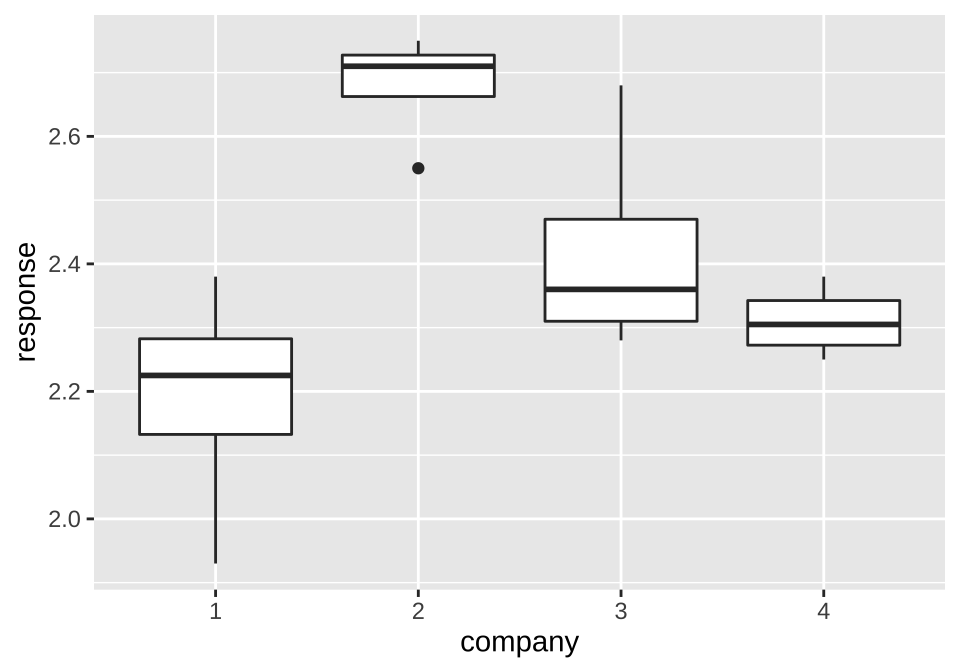
\includegraphics[width=.8\linewidth]{hierarchical_files/figure-latex/unnamed-chunk-12-1}

\begin{Shaded}
\begin{Highlighting}[]
\NormalTok{equatiomatic}\SpecialCharTok{::}\FunctionTok{extract\_eq}\NormalTok{(line1, }\AttributeTok{use\_coefs =} \ConstantTok{TRUE}\NormalTok{)}
\end{Highlighting}
\end{Shaded}

\[
\operatorname{\widehat{data\$SLE\_ALL\_AMT}} = 58.92 + 2.02(\operatorname{data\$MNF\_PCST})
\]

이제 모집단에서 매출액과 연간급여액에 대한 관계를 분석해 보자.

\begin{Shaded}
\begin{Highlighting}[]
\NormalTok{line2 }\OtherTok{\textless{}{-}} \FunctionTok{lm}\NormalTok{(data}\SpecialCharTok{$}\NormalTok{SLE\_ALL\_AMT }\SpecialCharTok{\textasciitilde{}}\NormalTok{ data}\SpecialCharTok{$}\NormalTok{MNF\_PCST)}
\FunctionTok{summary}\NormalTok{(line2)}
\end{Highlighting}
\end{Shaded}

\begin{verbatim}
## 
## Call:
## lm(formula = data$SLE_ALL_AMT ~ data$MNF_PCST)
## 
## Residuals:
##     Min      1Q  Median      3Q     Max 
## -3759.3   -52.0   -25.8    20.7  8228.3 
## 
## Coefficients:
##               Estimate Std. Error t value Pr(>|t|)    
## (Intercept)   58.92009    2.66787   22.09   <2e-16 ***
## data$MNF_PCST  2.01593    0.01018  197.94   <2e-16 ***
## ---
## Signif. codes:  0 '***' 0.001 '**' 0.01 '*' 0.05 '.' 0.1 ' ' 1
## 
## Residual standard error: 230.2 on 10165 degrees of freedom
## Multiple R-squared:  0.794,  Adjusted R-squared:  0.794 
## F-statistic: 3.918e+04 on 1 and 10165 DF,  p-value: < 2.2e-16
\end{verbatim}

\begin{Shaded}
\begin{Highlighting}[]
\FunctionTok{plot}\NormalTok{(data}\SpecialCharTok{$}\NormalTok{SLE\_ALL\_AMT }\SpecialCharTok{\textasciitilde{}}\NormalTok{ data}\SpecialCharTok{$}\NormalTok{MNF\_PCST, }\AttributeTok{xlab=}\StringTok{\textquotesingle{}연간급여액\textquotesingle{}}\NormalTok{, }\AttributeTok{ylab=}\StringTok{\textquotesingle{}매출액\textquotesingle{}}\NormalTok{)}
\FunctionTok{abline}\NormalTok{(line2, }\AttributeTok{col=}\StringTok{\textquotesingle{}red\textquotesingle{}}\NormalTok{)}
\end{Highlighting}
\end{Shaded}

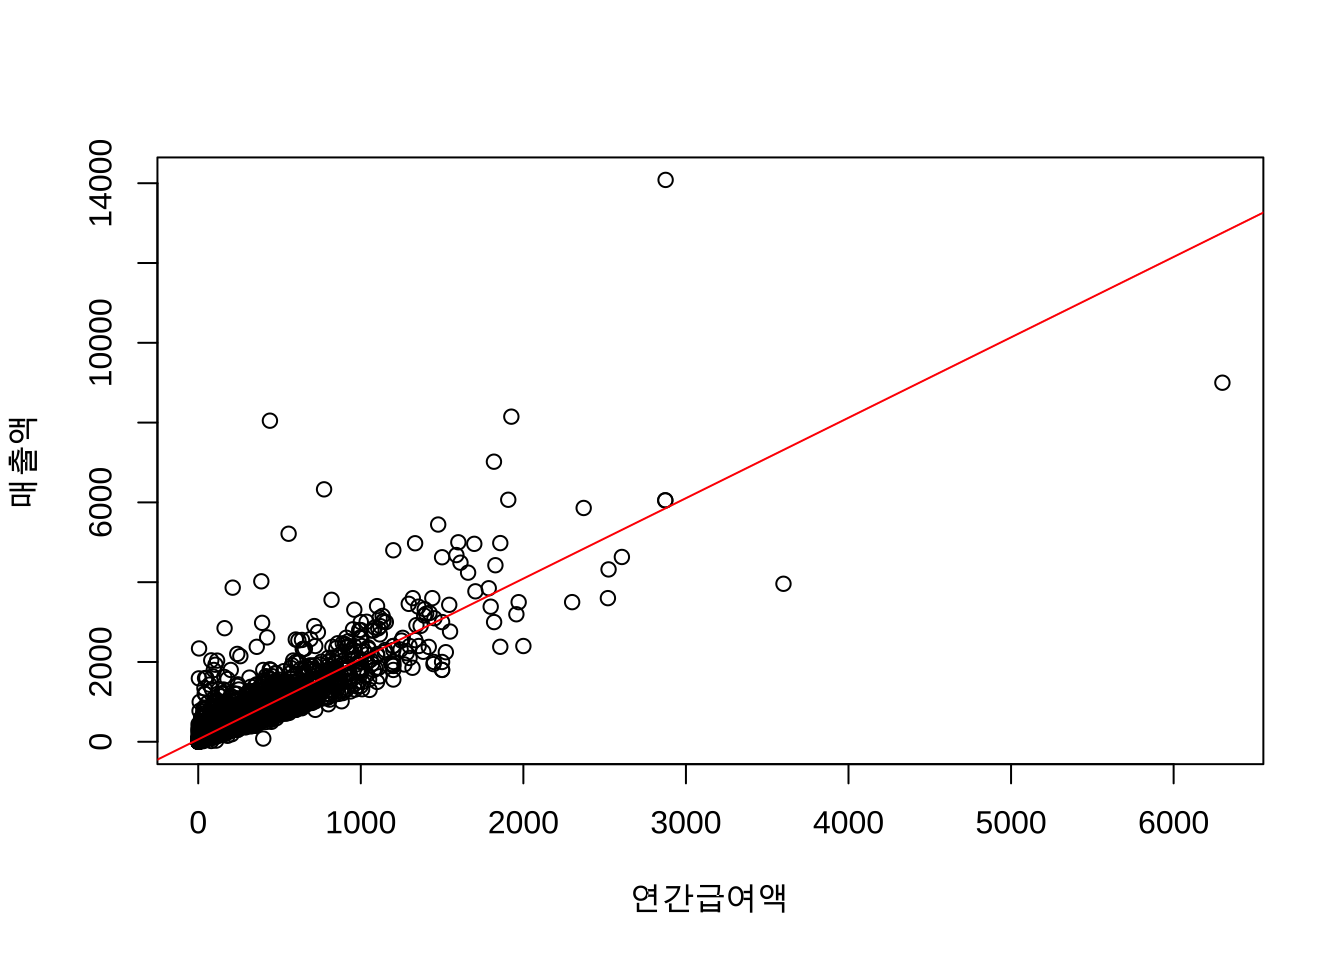
\includegraphics[width=.8\linewidth]{hierarchical_files/figure-latex/unnamed-chunk-14-1}

\begin{Shaded}
\begin{Highlighting}[]
\NormalTok{equatiomatic}\SpecialCharTok{::}\FunctionTok{extract\_eq}\NormalTok{(line2, }\AttributeTok{use\_coefs =} \ConstantTok{TRUE}\NormalTok{)}
\end{Highlighting}
\end{Shaded}

\[
\operatorname{\widehat{data\$SLE\_ALL\_AMT}} = 58.92 + 2.02(\operatorname{data\$MNF\_PCST})
\]

\hypertarget{uxd45cuxbcf8-uxbc30uxc815uxacfc-uxd45cuxbcf8-uxac00uxc911uxce58uxc744-uxc704uxd55c-uxd568uxc218}{%
\subsection{표본 배정과 표본 가중치을 위한 함수}\label{uxd45cuxbcf8-uxbc30uxc815uxacfc-uxd45cuxbcf8-uxac00uxc911uxce58uxc744-uxc704uxd55c-uxd568uxc218}}

\begin{Shaded}
\begin{Highlighting}[]
\CommentTok{\#표본 배정을 위한 함수}
\NormalTok{calsamspleize }\OtherTok{\textless{}{-}} \ControlFlowTok{function}\NormalTok{(samplesize, gugu) \{}
  \FunctionTok{ceiling}\NormalTok{(gugu}\SpecialCharTok{/}\FunctionTok{sum}\NormalTok{(gugu)}\SpecialCharTok{*}\NormalTok{samplesize)}
\NormalTok{\}}
\CommentTok{\#표본 가중치을 위한 함수}
\NormalTok{calweight2 }\OtherTok{\textless{}{-}} \ControlFlowTok{function}\NormalTok{(samplesize, gugu)\{}
\NormalTok{  xx }\OtherTok{\textless{}{-}} \FunctionTok{as.data.frame}\NormalTok{(gugu)}
\NormalTok{  yy }\OtherTok{\textless{}{-}} \FunctionTok{as.data.frame}\NormalTok{(samplesize)}
\NormalTok{  w }\OtherTok{=}\NormalTok{ xx}\SpecialCharTok{$}\NormalTok{Freq}\SpecialCharTok{/}\NormalTok{ yy}\SpecialCharTok{$}\NormalTok{Freq}
  \FunctionTok{data.frame}\NormalTok{(}\AttributeTok{AD\_CD =}\NormalTok{ xx}\SpecialCharTok{$}\NormalTok{Var1, }\AttributeTok{popN =}\NormalTok{ xx}\SpecialCharTok{$}\NormalTok{Freq, }\AttributeTok{samplesize =}\NormalTok{ yy}\SpecialCharTok{$}\NormalTok{Freq, }\AttributeTok{weight=}\NormalTok{w)}
\NormalTok{\}}
\end{Highlighting}
\end{Shaded}

\hypertarget{uxd45cuxbcf8-uxbc30uxc815}{%
\subsection{표본 배정}\label{uxd45cuxbcf8-uxbc30uxc815}}

\begin{Shaded}
\begin{Highlighting}[]
\CommentTok{\#먼저 1000 개의 표본을 비례할당}
\NormalTok{samplesize }\OtherTok{=} \DecValTok{1000} 
\NormalTok{sample.result }\OtherTok{\textless{}{-}} \FunctionTok{calsamspleize}\NormalTok{(samplesize, gugu)}

\CommentTok{\# 최소 표본을 1개로 지정 }
\NormalTok{sample.result }\OtherTok{\textless{}{-}}\NormalTok{ sample.result}\SpecialCharTok{+}\DecValTok{1}

\CommentTok{\# 표본 개수 다시 계산 }
\NormalTok{samplesize }\OtherTok{\textless{}{-}} \FunctionTok{sum}\NormalTok{(sample.result )}

\CommentTok{\# 표본의 총수}
\FunctionTok{sum}\NormalTok{(samplesize)}
\end{Highlighting}
\end{Shaded}

\begin{verbatim}
## [1] 1489
\end{verbatim}

\begin{Shaded}
\begin{Highlighting}[]
\CommentTok{\# 최종 표본 할당}
\FunctionTok{head}\NormalTok{(sample.result, }\AttributeTok{n=}\DecValTok{20}\NormalTok{)}
\end{Highlighting}
\end{Shaded}

\begin{verbatim}
## 
## 1101053 1101054 1101056 1101058 1101060 1101061 1101063 1101064 1101065 1101067 
##      12       4       4       3       5      28       7       5       5       4 
## 1101068 1101070 1101071 1101072 1102052 1102054 1102055 1102057 1102058 1102059 
##       3       3       3       3      14      10      20       6       4       7
\end{verbatim}

\hypertarget{uxd45cuxbcf8-uxac00uxc911uxce58-uxacc4uxc0b0-uxbc0f-uxbaa8uxc9d1uxb2e8-uxc815uxbcf4-uxc0dduxc131}{%
\subsection{표본 가중치 계산 및 모집단 정보 생성}\label{uxd45cuxbcf8-uxac00uxc911uxce58-uxacc4uxc0b0-uxbc0f-uxbaa8uxc9d1uxb2e8-uxc815uxbcf4-uxc0dduxc131}}

\begin{Shaded}
\begin{Highlighting}[]
\NormalTok{popinfo }\OtherTok{\textless{}{-}} \FunctionTok{calweight2}\NormalTok{(sample.result, gugu)}
\FunctionTok{head}\NormalTok{(popinfo)}
\end{Highlighting}
\end{Shaded}

\begin{verbatim}
##     AD_CD popN samplesize   weight
## 1 1101053  111         12 9.250000
## 2 1101054   23          4 5.750000
## 3 1101056   22          4 5.500000
## 4 1101058   11          3 3.666667
## 5 1101060   33          5 6.600000
## 6 1101061  274         28 9.785714
\end{verbatim}

\hypertarget{uxc790uxb8ccuxc640-uxbaa8uxc9d1uxb2e8-uxc815uxbcf4uxc758-uxacb0uxd569}{%
\subsection{자료와 모집단 정보의 결합}\label{uxc790uxb8ccuxc640-uxbaa8uxc9d1uxb2e8-uxc815uxbcf4uxc758-uxacb0uxd569}}

\begin{Shaded}
\begin{Highlighting}[]
\NormalTok{data1 }\OtherTok{\textless{}{-}} \FunctionTok{left\_join}\NormalTok{(data,popinfo,}\AttributeTok{by=}\StringTok{"AD\_CD"}\NormalTok{)  }
\FunctionTok{head}\NormalTok{(data1, }\AttributeTok{n=}\DecValTok{20}\NormalTok{)}
\end{Highlighting}
\end{Shaded}

\begin{verbatim}
## # A tibble: 20 x 7
## # Rowwise: 
##    SURV_PHS_SLR_SUM SLE_ALL_AMT MNF_PCST AD_CD    popN samplesize weight
##               <dbl>       <dbl>    <dbl> <fct>   <int>      <dbl>  <dbl>
##  1               14         103       23 1101053   111         12   9.25
##  2               13          40       16 1101053   111         12   9.25
##  3                4          40       15 1101053   111         12   9.25
##  4               12         100       38 1101053   111         12   9.25
##  5                2          20        8 1101053   111         12   9.25
##  6                7          36       14 1101053   111         12   9.25
##  7                1          30        9 1101053   111         12   9.25
##  8                7          15        6 1101053   111         12   9.25
##  9                2          15        6 1101053   111         12   9.25
## 10                5          56       15 1101053   111         12   9.25
## 11                7          22        8 1101053   111         12   9.25
## 12                9          54       21 1101053   111         12   9.25
## 13               11         100       70 1101053   111         12   9.25
## 14               15          76       24 1101053   111         12   9.25
## 15               13          43       10 1101053   111         12   9.25
## 16                7          43        9 1101053   111         12   9.25
## 17                7          43        9 1101053   111         12   9.25
## 18               13          70       32 1101053   111         12   9.25
## 19               16         100       38 1101053   111         12   9.25
## 20               11          90       35 1101053   111         12   9.25
\end{verbatim}

\hypertarget{uxb9e4uxcd9cuxc561uxc758-uxc9c0uxc5eduxbcc4-uxbaa8uxc9d1uxb2e8-uxd3c9uxade0uxacc4uxc0b0}{%
\subsection{매출액의 지역별 모집단 평균계산}\label{uxb9e4uxcd9cuxc561uxc758-uxc9c0uxc5eduxbcc4-uxbaa8uxc9d1uxb2e8-uxd3c9uxade0uxacc4uxc0b0}}

\begin{Shaded}
\begin{Highlighting}[]
\NormalTok{popMeanT }\OtherTok{\textless{}{-}}\NormalTok{ data1 }\SpecialCharTok{\%\textgreater{}\%} \FunctionTok{group\_by}\NormalTok{(AD\_CD)   }\SpecialCharTok{\%\textgreater{}\%}  
  \FunctionTok{summarise}\NormalTok{(}\AttributeTok{SLE\_ALL\_AMT\_mean  =} \FunctionTok{mean}\NormalTok{(SLE\_ALL\_AMT, }\AttributeTok{na.rm=}\ConstantTok{TRUE}\NormalTok{)) }\SpecialCharTok{\%\textgreater{}\%} \FunctionTok{as.data.frame}\NormalTok{()}
\FunctionTok{head}\NormalTok{(popMeanT)}
\end{Highlighting}
\end{Shaded}

\begin{verbatim}
##     AD_CD SLE_ALL_AMT_mean
## 1 1101053         474.3514
## 2 1101054         583.4348
## 3 1101056         479.0000
## 4 1101058         254.6364
## 5 1101060         319.1818
## 6 1101061         373.5182
\end{verbatim}

\hypertarget{uxd45cuxbcf8-uxcd94uxcd9c}{%
\subsection{표본 추출}\label{uxd45cuxbcf8-uxcd94uxcd9c}}

\begin{Shaded}
\begin{Highlighting}[]
\NormalTok{sample.final }\OtherTok{=}\NormalTok{ sampling}\SpecialCharTok{::}\FunctionTok{strata}\NormalTok{(data1 , }\StringTok{\textquotesingle{}AD\_CD\textquotesingle{}}\NormalTok{, }\AttributeTok{size=}\NormalTok{sample.result, }\AttributeTok{method=}\StringTok{"srswor"}\NormalTok{)}
\NormalTok{sampledata }\OtherTok{=}\NormalTok{ data1[sample.final}\SpecialCharTok{$}\NormalTok{ID\_unit, ] }
\NormalTok{sampledata }\OtherTok{\textless{}{-}} \FunctionTok{as.data.frame}\NormalTok{(sampledata )}
\FunctionTok{head}\NormalTok{(sampledata, }\AttributeTok{n=}\DecValTok{20}\NormalTok{)}
\end{Highlighting}
\end{Shaded}

\begin{verbatim}
##    SURV_PHS_SLR_SUM SLE_ALL_AMT MNF_PCST   AD_CD popN samplesize weight
## 1                 7          22        8 1101053  111         12   9.25
## 2                 7          43        9 1101053  111         12   9.25
## 3                 1           3        1 1101053  111         12   9.25
## 4                 3          12        5 1101053  111         12   9.25
## 5                43         298       99 1101053  111         12   9.25
## 6                73         298       69 1101053  111         12   9.25
## 7                16         210      120 1101053  111         12   9.25
## 8                90         781      429 1101053  111         12   9.25
## 9               100         600       20 1101053  111         12   9.25
## 10               10          24        7 1101053  111         12   9.25
## 11              192         520      180 1101053  111         12   9.25
## 12              222        1208      733 1101053  111         12   9.25
## 13               61         420      189 1101054   23          4   5.75
## 14              138         800      320 1101054   23          4   5.75
## 15              288        1020      357 1101054   23          4   5.75
## 16              768        2380      360 1101054   23          4   5.75
## 17               20         144       70 1101056   22          4   5.50
## 18                5         117       60 1101056   22          4   5.50
## 19               10         155       30 1101056   22          4   5.50
## 20              151         365      150 1101056   22          4   5.50
\end{verbatim}

\hypertarget{uxd45cuxbcf8uxc790uxb8ccuxc640-uxd45cuxbcf8-uxcd94uxcd9cuxc815uxbcf4-uxacb0uxd569}{%
\subsection{표본자료와 표본 추출정보 결합}\label{uxd45cuxbcf8uxc790uxb8ccuxc640-uxd45cuxbcf8-uxcd94uxcd9cuxc815uxbcf4-uxacb0uxd569}}

\begin{Shaded}
\begin{Highlighting}[]
\NormalTok{strat\_design }\OtherTok{\textless{}{-}} \FunctionTok{svydesign}\NormalTok{(}\AttributeTok{id =} \SpecialCharTok{\textasciitilde{}}\DecValTok{1}\NormalTok{, }\AttributeTok{strata =} \SpecialCharTok{\textasciitilde{}}\NormalTok{AD\_CD, }\AttributeTok{weights =} \SpecialCharTok{\textasciitilde{}}\NormalTok{weight, }\AttributeTok{data =}\NormalTok{ sampledata)}
\end{Highlighting}
\end{Shaded}

\hypertarget{uxb2e8uxc21c-uxcd94uxc815uxb7c9-uxacc4uxc0b0}{%
\subsection{단순 추정량 계산}\label{uxb2e8uxc21c-uxcd94uxc815uxb7c9-uxacc4uxc0b0}}

\begin{Shaded}
\begin{Highlighting}[]
\NormalTok{res0 }\OtherTok{\textless{}{-}}\NormalTok{ survey}\SpecialCharTok{::}\FunctionTok{svyby}\NormalTok{(}\SpecialCharTok{\textasciitilde{}}\NormalTok{SLE\_ALL\_AMT, }\SpecialCharTok{\textasciitilde{}}\NormalTok{AD\_CD, strat\_design, svymean)}
\FunctionTok{head}\NormalTok{(res0, }\AttributeTok{n=}\DecValTok{20}\NormalTok{)}
\end{Highlighting}
\end{Shaded}

\begin{verbatim}
##           AD_CD SLE_ALL_AMT         se
## 1101053 1101053   334.91667 109.349485
## 1101054 1101054  1155.00000 426.722002
## 1101056 1101056   195.25000  57.143642
## 1101058 1101058    76.66667   8.333333
## 1101060 1101060   260.40000  77.576156
## 1101061 1101061   493.14286  99.047270
## 1101063 1101063   233.57143  39.544343
## 1101064 1101064   243.60000  58.795918
## 1101065 1101065   228.40000  58.707410
## 1101067 1101067   215.25000  81.787708
## 1101068 1101068    75.00000  24.637370
## 1101070 1101070    59.33333  16.895101
## 1101071 1101071   360.00000  83.266640
## 1101072 1101072   756.33333 345.904772
## 1102052 1102052   459.71429 100.088720
## 1102054 1102054   319.90000 149.510271
## 1102055 1102055   682.40000 133.417082
## 1102057 1102057   211.66667  66.352928
## 1102058 1102058   499.00000 235.047158
## 1102059 1102059   389.42857 151.791501
\end{verbatim}

\hypertarget{uxbcf4uxc870uxbcc0uxc218uxc5d0-uxb300uxd55c-uxce35uxbcc4-uxbaa8uxd3c9uxade0-uxacc4uxc0b0}{%
\subsection{보조변수에 대한 층별 모평균 계산}\label{uxbcf4uxc870uxbcc0uxc218uxc5d0-uxb300uxd55c-uxce35uxbcc4-uxbaa8uxd3c9uxade0-uxacc4uxc0b0}}

\begin{Shaded}
\begin{Highlighting}[]
\NormalTok{popMean }\OtherTok{\textless{}{-}}\NormalTok{ data1 }\SpecialCharTok{\%\textgreater{}\%} \FunctionTok{group\_by}\NormalTok{(AD\_CD)   }\SpecialCharTok{\%\textgreater{}\%}  
  \FunctionTok{summarise}\NormalTok{(}\AttributeTok{MNF\_PCST\_mean  =} \FunctionTok{mean}\NormalTok{(MNF\_PCST, }\AttributeTok{na.rm=}\ConstantTok{TRUE}\NormalTok{),  }\AttributeTok{SURV\_PHS\_SLR\_SUM\_mean=}\FunctionTok{mean}\NormalTok{(SURV\_PHS\_SLR\_SUM, }\AttributeTok{na.rm=}\ConstantTok{TRUE}\NormalTok{)) }\SpecialCharTok{\%\textgreater{}\%} \FunctionTok{as.data.frame}\NormalTok{()}
\FunctionTok{head}\NormalTok{(popMean)}
\end{Highlighting}
\end{Shaded}

\begin{verbatim}
##     AD_CD MNF_PCST_mean SURV_PHS_SLR_SUM_mean
## 1 1101053      214.2883              85.09009
## 2 1101054      217.2609             144.69565
## 3 1101056      205.8636             121.54545
## 4 1101058      130.5455              33.81818
## 5 1101060      135.4848              76.81818
## 6 1101061      157.2007              77.51095
\end{verbatim}

\hypertarget{uxce35uxbcc4-uxc0acuxc5c5uxccb4-uxc218-uxc0dduxc131}{%
\subsection{층별 사업체 수 생성}\label{uxce35uxbcc4-uxc0acuxc5c5uxccb4-uxc218-uxc0dduxc131}}

\begin{Shaded}
\begin{Highlighting}[]
\NormalTok{popN }\OtherTok{\textless{}{-}}\NormalTok{ popinfo[,}\DecValTok{1}\SpecialCharTok{:}\DecValTok{2}\NormalTok{]}
\FunctionTok{head}\NormalTok{(popN)}
\end{Highlighting}
\end{Shaded}

\begin{verbatim}
##     AD_CD popN
## 1 1101053  111
## 2 1101054   23
## 3 1101056   22
## 4 1101058   11
## 5 1101060   33
## 6 1101061  274
\end{verbatim}

\hypertarget{uxc18cuxc9c0uxc5ed-uxbaa8uxd615-uxc801uxd569}{%
\subsection{소지역 모형 적합}\label{uxc18cuxc9c0uxc5ed-uxbaa8uxd615-uxc801uxd569}}

\begin{Shaded}
\begin{Highlighting}[]
\NormalTok{res }\OtherTok{\textless{}{-}} \FunctionTok{eblupBHF}\NormalTok{(SLE\_ALL\_AMT }\SpecialCharTok{\textasciitilde{}}\NormalTok{ MNF\_PCST }\SpecialCharTok{+}\NormalTok{ SURV\_PHS\_SLR\_SUM, }\AttributeTok{dom =}\NormalTok{AD\_CD, }\AttributeTok{meanxpop =}\NormalTok{ popMean, }
                \AttributeTok{popnsize =}\NormalTok{ popN, }\AttributeTok{data =}\NormalTok{ sampledata)}
\end{Highlighting}
\end{Shaded}

\hypertarget{uxbaa8uxc218-uxcd94uxc815-uxacb0uxacfc}{%
\subsection{모수 추정 결과}\label{uxbaa8uxc218-uxcd94uxc815-uxacb0uxacfc}}

\[ \hat \sigma^2_b =49.65, \quad \hat \sigma^2_e = 17216.15 \]

\begin{Shaded}
\begin{Highlighting}[]
\NormalTok{res}\SpecialCharTok{$}\NormalTok{fit}\SpecialCharTok{$}\NormalTok{summary}
\end{Highlighting}
\end{Shaded}

\begin{verbatim}
## Linear mixed model fit by REML ['lmerMod']
## Formula: ys ~ -1 + Xs + (1 | dom)
## 
## REML criterion at convergence: 18756.5
## 
## Scaled residuals: 
##     Min      1Q  Median      3Q     Max 
## -6.3258 -0.2029 -0.0063  0.2039 20.8385 
## 
## Random effects:
##  Groups   Name        Variance Std.Dev.
##  dom      (Intercept)    49.66   7.047 
##  Residual             17216.15 131.210 
## Number of obs: 1489, groups:  dom, 326
## 
## Fixed effects:
##                    Estimate Std. Error t value
## Xs(Intercept)       5.74487    4.00677   1.434
## XsMNF_PCST          1.24440    0.02233  55.721
## XsSURV_PHS_SLR_SUM  2.45568    0.04966  49.455
## 
## Correlation of Fixed Effects:
##             Xs(In) XMNF_P
## XsMNF_PCST  -0.159       
## XSURV_PHS_S -0.191 -0.771
\end{verbatim}

\hypertarget{uxcd94uxc815uxb7c9uxc758-uxbe44uxad50}{%
\subsection{추정량의 비교}\label{uxcd94uxc815uxb7c9uxc758-uxbe44uxad50}}

\begin{Shaded}
\begin{Highlighting}[]
\NormalTok{finalres1 }\OtherTok{\textless{}{-}}\NormalTok{ popMeanT}
\NormalTok{finalres1}\SpecialCharTok{$}\NormalTok{samplemean }\OtherTok{\textless{}{-}}\NormalTok{ res0}\SpecialCharTok{$}\NormalTok{SLE\_ALL\_AMT}
\NormalTok{finalres1}\SpecialCharTok{$}\NormalTok{sae }\OtherTok{\textless{}{-}}\NormalTok{ res}\SpecialCharTok{$}\NormalTok{eblup}\SpecialCharTok{$}\NormalTok{eblup}
\NormalTok{finalres1 }\OtherTok{\textless{}{-}}\NormalTok{ finalres1[}\FunctionTok{order}\NormalTok{(finalres1}\SpecialCharTok{$}\NormalTok{SLE\_ALL\_AMT\_mean), ]}
\NormalTok{finalres1}\SpecialCharTok{$}\NormalTok{area }\OtherTok{\textless{}{-}} \DecValTok{1}\SpecialCharTok{:}\NormalTok{(}\FunctionTok{dim}\NormalTok{(finalres1)[}\DecValTok{1}\NormalTok{])}
\FunctionTok{colnames}\NormalTok{(finalres1) }\OtherTok{\textless{}{-}} \FunctionTok{c}\NormalTok{(}\StringTok{"AD\_CD"}\NormalTok{, }\StringTok{"실제평균"}\NormalTok{, }\StringTok{"표본평균"}\NormalTok{, }\StringTok{"소지역추정량"}\NormalTok{, }\StringTok{"AREA"}\NormalTok{)}
\NormalTok{finalres1 }\OtherTok{\textless{}{-}}\NormalTok{ finalres1[,}\DecValTok{2}\SpecialCharTok{:}\DecValTok{5}\NormalTok{]}
\NormalTok{finalres2 }\OtherTok{\textless{}{-}} \FunctionTok{gather}\NormalTok{(finalres1,  Type, Estimates,}\StringTok{"실제평균"}\NormalTok{, }\StringTok{"표본평균"}\NormalTok{, }\StringTok{"소지역추정량"}\NormalTok{)}
\end{Highlighting}
\end{Shaded}

\begin{Shaded}
\begin{Highlighting}[]
\FunctionTok{ggplot}\NormalTok{(finalres2, }\FunctionTok{aes}\NormalTok{(}\AttributeTok{x=}\NormalTok{AREA, }\AttributeTok{y=}\NormalTok{Estimates, }\AttributeTok{color=}\NormalTok{Type)) }\SpecialCharTok{+}\FunctionTok{geom\_line}\NormalTok{()}
\end{Highlighting}
\end{Shaded}

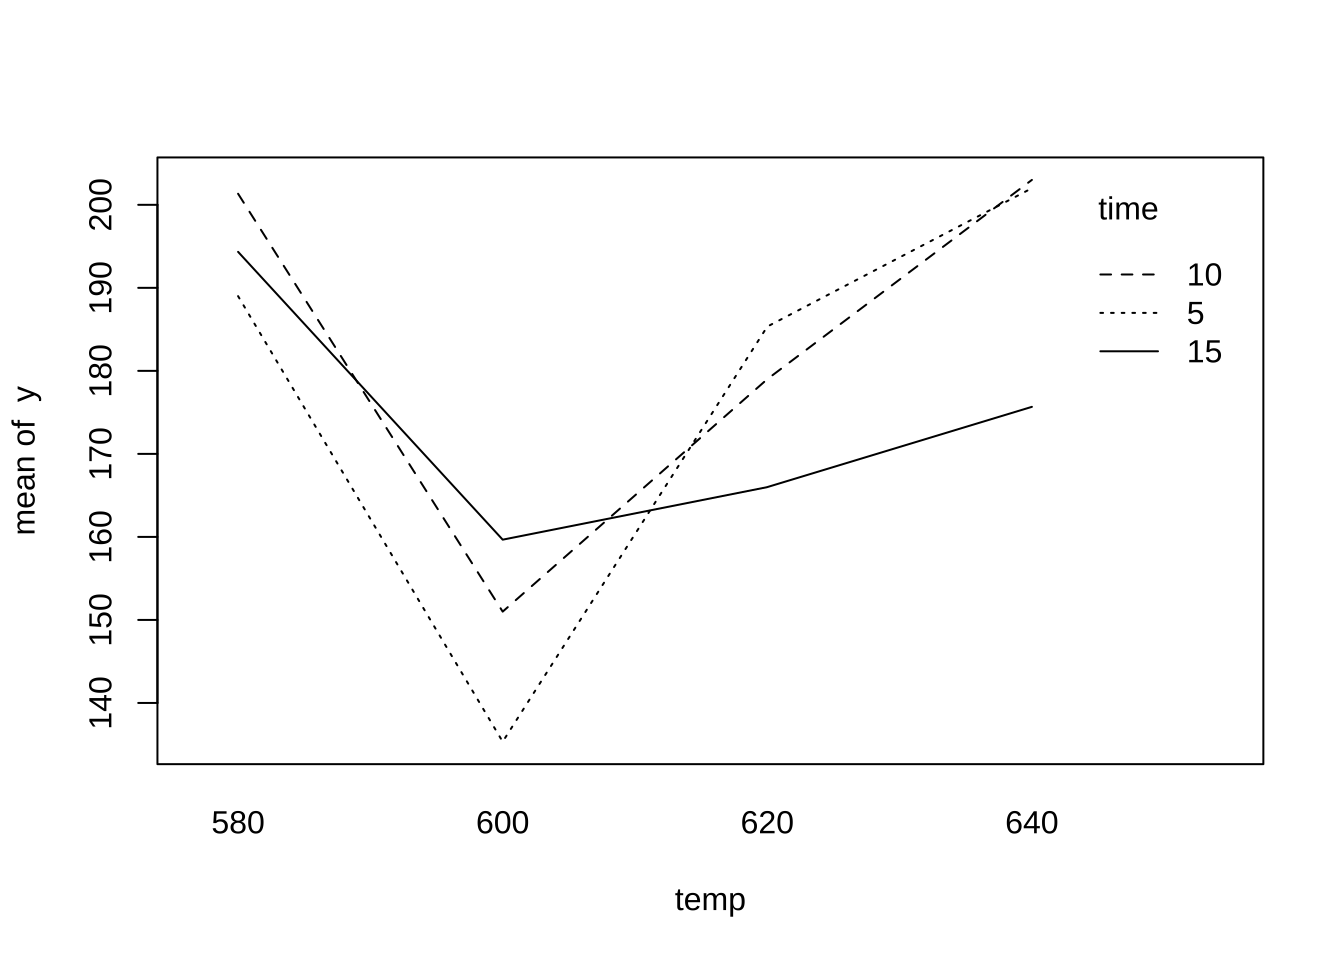
\includegraphics{hierarchical_files/figure-latex/unnamed-chunk-29-1.pdf}

\begin{Shaded}
\begin{Highlighting}[]
\NormalTok{finalres3 }\OtherTok{\textless{}{-}}\NormalTok{ finalres2 }\SpecialCharTok{\%\textgreater{}\%} \FunctionTok{filter}\NormalTok{(Type }\SpecialCharTok{!=} \StringTok{"표본평균"}\NormalTok{)}
\FunctionTok{ggplot}\NormalTok{(finalres3, }\FunctionTok{aes}\NormalTok{(}\AttributeTok{x=}\NormalTok{AREA, }\AttributeTok{y=}\NormalTok{Estimates, }\AttributeTok{color=}\NormalTok{Type)) }\SpecialCharTok{+}\FunctionTok{geom\_line}\NormalTok{()}
\end{Highlighting}
\end{Shaded}

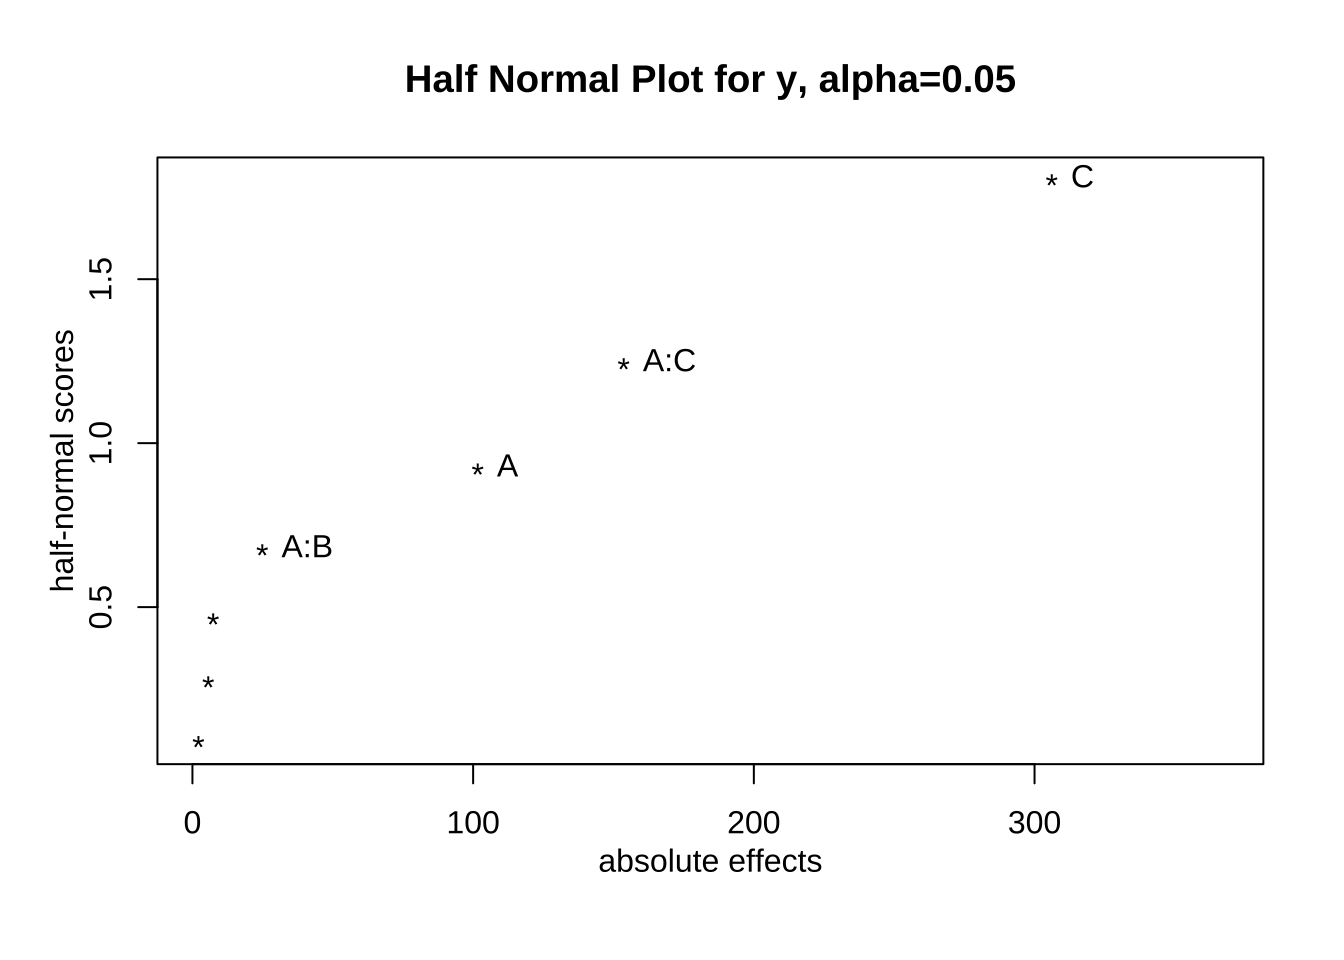
\includegraphics{hierarchical_files/figure-latex/unnamed-chunk-30-1.pdf}

\hypertarget{school}{%
\chapter{계층모형}\label{school}}

이제 계층모형에 대한 전현적인 예제와 분석을 살펴보고자 한다. 아래에서 사용할 자료와 분석 내용은
교과서 \citep{finch2019multilevel}를 따른 것이다.

\hypertarget{uxd559uxc0dd-uxc131uxcde8uxb3c4-uxc790uxb8cc}{%
\section{학생 성취도 자료}\label{uxd559uxc0dd-uxc131uxcde8uxb3c4-uxc790uxb8cc}}

학생 선취도 자료는 교과서 \citep{finch2019multilevel} 의 \href{http://www.mlminr.com/}{홈페이지}에서 다운로드 받을 수 있다.

\begin{Shaded}
\begin{Highlighting}[]
\NormalTok{Achieve }\OtherTok{\textless{}{-}} \FunctionTok{read.csv}\NormalTok{(}\StringTok{"Achieve.csv"}\NormalTok{, }\AttributeTok{header=}\NormalTok{T)}
\FunctionTok{head}\NormalTok{(Achieve,}\AttributeTok{n=}\DecValTok{3}\NormalTok{)}
\end{Highlighting}
\end{Shaded}

\begin{verbatim}
##   row id region corp school class gender age race geread gevocab gereadcm
## 1   1  1      2  940    767     1      2 104    5    3.5     3.1      3.2
## 2   2  2      2  940    767     1      2 106    5    1.2     2.8      2.0
## 3   3  3      2  940    767     1      2 112    5    2.1     1.7      1.9
##   gelang gelangmc gelangcm gemath gemathcp gemathcm getotal npanverb npamem
## 1    2.3      4.3      3.0    3.1      2.7      2.9     3.0       16     56
## 2    1.8      1.7      1.6    3.2      4.3      3.8     2.7       39     79
## 3    2.5      2.2      2.4    3.6      3.2      3.4     2.7       37     41
##   npaverb npatotal csi multi clenroll classize ptratio ptia locale chapter1
## 1      46       26  90     2       16        1      16    2      7        1
## 2      37       47  99     2       16        1      16    2      7        1
## 3      34       35  94     2       16        1      16    2      7        1
##    ses context calender senroll sattend white1 black1 hispanc1 asian1 aindian1
## 1 80.4     929        1     463    95.6   99.8      0        0      0        0
## 2 80.4     929        1     463    95.6   99.8      0        0      0        0
## 3 80.4     929        1     463    95.6   99.8      0        0      0        0
##   multi1 total1 noteach avgage1 avgexp1 avgsal1 spert thrdclss thrdstud passla1
## 1    0.2    0.2    28.5    46.2    20.6   43517  16.3        4       60      63
## 2    0.2    0.2    28.5    46.2    20.6   43517  16.3        4       60      63
## 3    0.2    0.2    28.5    46.2    20.6   43517  16.3        4       60      63
##   passmth1 passbth1 tmnnce1 rmdnce1 lamdnce1 mmdnce1 tmdnce1 avgcsi1 geog
## 1       74       52    60.5    57.6       55      61    59.7      99    2
## 2       74       52    60.5    57.6       55      61    59.7      99    2
## 3       74       52    60.5    57.6       55      61    59.7      99    2
##   totepp cenroll cattend freelnch lep speced minority white2 black2 hispanc2
## 1   5956    3115    95.9       16 0.2   14.4      1.2   3077      1       12
## 2   5956    3115    95.9       16 0.2   14.4      1.2   3077      1       12
## 3   5956    3115    95.9       16 0.2   14.4      1.2   3077      1       12
##   asian2 aindian2 multi2 total2 thrdadm thrdtech avgage2 avgexp2 avgsal2
## 1      3        1     21     38     208       11    45.2    18.4   41096
## 2      3        1     21     38     208       11    45.2    18.4   41096
## 3      3        1     21     38     208       11    45.2    18.4   41096
##   thrdaide passla2 passmth2 passbth2 tmnnce2 rmdnce2 lamdnce2 mmdnce2 tmdnce2
## 1        3      67       70       52    59.4    57.8     59.8    60.6    60.8
## 2        3      67       70       52    59.4    57.8     59.8    60.6    60.8
## 3        3      67       70       52    59.4    57.8     59.8    60.6    60.8
##   rmediate
## 1       18
## 2       18
## 3       18
\end{verbatim}

성취도 자료 \texttt{Achieve}는 160개 학교를 추출하고 각 학교마다 작게는 11명, 크게는 162명의 학생들을 추출하여 학교의 여러 가지 정보와 학생들의 다양한 성적을 수집한 자료이다.

성취도 자료 \texttt{Achieve}는 계층적 자료이며 다음과 같은 계층구조를 가지고 있다.

\begin{itemize}
\tightlist
\item
  계층 1 : 학생
\item
  계층 2 : 학교
\end{itemize}

분석의 목적은 학교의 특성과 학생들의 다양한 성적들(예를 들어 어휘 능력, vocabulary scores)이 학생들의 읽기 성취도(general reading achievement)에 어떤 영향을 미치는지 분석하는 것이다.

이제 \(i\) 번째 학교에 속한 \(j\) 번쨰 학생의 읽기 성취도 점수를 \(y_{ij}\) 라고 하자.

\hypertarget{uxb2e8uxc21c-uxacc4uxce35uxbaa8uxd615}{%
\section{단순 계층모형}\label{uxb2e8uxc21c-uxacc4uxce35uxbaa8uxd615}}

가장 단순한 계층 모형으로서 읽기 성취도 점수에 대하여 학교 \texttt{school} 이 임의효과인 모형을 고려해 보자.

\begin{equation}
y_{ij} = \beta_0 + b_{0i} + e_{ij}
\label{eq:multimodel1}
\end{equation}

위의 식에서 \(\beta_0\) 는 전체 평균 점수를 나타내는 모수이며 학교에 대한 임의효과 \(b_{0i}\) 와 오차항 \(e_{ij}\) 는 서로 독립이며 다음과 같은 분포를 따른다.

\[ b_{0i} \sim N(0, \sigma_{b0}^2 ) , \quad e_{ij} \sim N(0, \sigma_e^2) \]
이제 \texttt{lmer} 함수로 모형 \eqref{eq:multimodel1}을 적합시켜 보자.

\begin{Shaded}
\begin{Highlighting}[]
\NormalTok{model1 }\OtherTok{\textless{}{-}} \FunctionTok{lmer}\NormalTok{(geread}\SpecialCharTok{\textasciitilde{}}\DecValTok{1} \SpecialCharTok{+}\NormalTok{(}\DecValTok{1}\SpecialCharTok{|}\NormalTok{school), }\AttributeTok{data=}\NormalTok{Achieve)}
\FunctionTok{summary}\NormalTok{(model1)}
\end{Highlighting}
\end{Shaded}

\begin{verbatim}
## Linear mixed model fit by REML. t-tests use Satterthwaite's method [
## lmerModLmerTest]
## Formula: geread ~ 1 + (1 | school)
##    Data: Achieve
## 
## REML criterion at convergence: 46268.3
## 
## Scaled residuals: 
##     Min      1Q  Median      3Q     Max 
## -2.3229 -0.6378 -0.2138  0.2850  3.8812 
## 
## Random effects:
##  Groups   Name        Variance Std.Dev.
##  school   (Intercept) 0.3915   0.6257  
##  Residual             5.0450   2.2461  
## Number of obs: 10320, groups:  school, 160
## 
## Fixed effects:
##              Estimate Std. Error        df t value Pr(>|t|)    
## (Intercept)   4.30675    0.05498 158.53888   78.34   <2e-16 ***
## ---
## Signif. codes:  0 '***' 0.001 '**' 0.01 '*' 0.05 '.' 0.1 ' ' 1
\end{verbatim}

\begin{Shaded}
\begin{Highlighting}[]
\NormalTok{equatiomatic}\SpecialCharTok{::}\FunctionTok{extract\_eq}\NormalTok{(model1, }\AttributeTok{use\_coefs =} \ConstantTok{TRUE}\NormalTok{)}
\end{Highlighting}
\end{Shaded}

\[
\begin{aligned}
  \operatorname{\widehat{geread}}_{i}  &\sim N \left(4.31_{\alpha_{j[i]}}, \sigma^2 \right) \\
    \alpha_{j}  &\sim N \left(0, 0.63 \right)
    \text{, for school j = 1,} \dots \text{,J}
\end{aligned}
\]

추정결과를 보면 학생들의 읽기 성취도의 전체 평의 추정량은 \(\hat \beta_0= 4.3067534\)이다.
임의효과의 분산성분 \(\sigma_{b0}\) 과 오차항의 븐산 \(\sigma_e\)의 추정량은 다음과 같다.

\[ \hat {\sigma}_{b0} = 0.6257119 , \quad
\hat {\sigma}_{e} = 2.2461096 \]

지난 강의에서 언급한 그룹내 상관계수(ICC)의 값을 구해보면 0.072 로서 같은 학교에 속한 학생들의 성적들의 상관계수를 의미한다.

\[ \text{ICC } = \frac{\hat {\sigma}^2_{b0} }{\hat {\sigma}^2_{b0} + \hat {\sigma}^2_{e}  }
 = 0.072 \]

\hypertarget{uxacc4uxce35-1-uxc124uxba85uxbcc0uxc218uxac00-uxc788uxb294-uxbaa8uxd615}{%
\section{계층 1 설명변수가 있는 모형}\label{uxacc4uxce35-1-uxc124uxba85uxbcc0uxc218uxac00-uxc788uxb294-uxbaa8uxd615}}

이제 학생들의 어휘능력 성적 \texttt{gevocab}를 설명 변수(\(x_{ij1}\))로 포함하는 모형을 고려해 보자.
첫 번째 계층의 구성원인 학생들에 대한 성적이므로 \textbf{계층 1 설명변수(level 1 covariate)}라고 부른다.
일단 어휘능력 성적은 고정 효과로서 모집단 전체에 대한 회귀 계수를 나타낸다.

\begin{equation}
y_{ij} = (\beta_0 + b_{0i}) + \beta_1 x_{ij1} + e_{ij}
\label{eq:multimodel11}
\end{equation}

\begin{Shaded}
\begin{Highlighting}[]
\NormalTok{model11 }\OtherTok{\textless{}{-}} \FunctionTok{lmer}\NormalTok{(geread}\SpecialCharTok{\textasciitilde{}}\NormalTok{gevocab }\SpecialCharTok{+}\NormalTok{(}\DecValTok{1}\SpecialCharTok{|}\NormalTok{school), }\AttributeTok{data=}\NormalTok{Achieve)}
\FunctionTok{summary}\NormalTok{(model11)}
\end{Highlighting}
\end{Shaded}

\begin{verbatim}
## Linear mixed model fit by REML. t-tests use Satterthwaite's method [
## lmerModLmerTest]
## Formula: geread ~ gevocab + (1 | school)
##    Data: Achieve
## 
## REML criterion at convergence: 43137.2
## 
## Scaled residuals: 
##     Min      1Q  Median      3Q     Max 
## -3.0823 -0.5735 -0.2103  0.3207  4.4334 
## 
## Random effects:
##  Groups   Name        Variance Std.Dev.
##  school   (Intercept) 0.09978  0.3159  
##  Residual             3.76647  1.9407  
## Number of obs: 10320, groups:  school, 160
## 
## Fixed effects:
##              Estimate Std. Error        df t value Pr(>|t|)    
## (Intercept) 2.023e+00  4.931e-02 7.582e+02   41.03   <2e-16 ***
## gevocab     5.129e-01  8.373e-03 9.801e+03   61.26   <2e-16 ***
## ---
## Signif. codes:  0 '***' 0.001 '**' 0.01 '*' 0.05 '.' 0.1 ' ' 1
## 
## Correlation of Fixed Effects:
##         (Intr)
## gevocab -0.758
\end{verbatim}

학생들의 어휘능력 성적은 읽기 성취도를 예측하는데 유의한 변수임이 t-검정로 나타난다(t-통계량 = 61.26). 또한 다음의 추정식과 같이 어휘능력 성적이 1점 증가하면 평균적으로 읽기 성취도은 0.5점 증가한다.

\begin{Shaded}
\begin{Highlighting}[]
\NormalTok{equatiomatic}\SpecialCharTok{::}\FunctionTok{extract\_eq}\NormalTok{(model11, }\AttributeTok{use\_coefs =} \ConstantTok{TRUE}\NormalTok{)}
\end{Highlighting}
\end{Shaded}

\[
\begin{aligned}
  \operatorname{\widehat{geread}}_{i}  &\sim N \left(2.02_{\alpha_{j[i]}} + 0.51_{\beta_{1}}(\operatorname{gevocab}), \sigma^2 \right) \\
    \alpha_{j}  &\sim N \left(0, 0.32 \right)
    \text{, for school j = 1,} \dots \text{,J}
\end{aligned}
\]

\hypertarget{uxacc4uxce35-2-uxc124uxba85uxbcc0uxc218uxac00-uxc788uxb294-uxbaa8uxd615}{%
\section{계층 2 설명변수가 있는 모형}\label{uxacc4uxce35-2-uxc124uxba85uxbcc0uxc218uxac00-uxc788uxb294-uxbaa8uxd615}}

이제 학교의 규모를 나타내는 등록 학생의 수 \texttt{senroll}를 설명 변수(\(x_{i2}\))로 포함하는 모형을 고려해 보자. 두 번째 계층의 구성원인 학교들에 대한 정보이므로 \textbf{계층 2 설명변수(level 2 covariate)}라고 부른다. 일단 등록 학생의 수은 고정 효과로서 모집단 전체에 대한 회귀 계수를 나타낸다.

\begin{equation}
y_{ij} = (\beta_0 + b_{0i}) + \beta_1 x_{ij1} + \beta_2 x_{i2} + e_{ij}
\label{eq:multimodel12}
\end{equation}

\begin{Shaded}
\begin{Highlighting}[]
\NormalTok{model12 }\OtherTok{\textless{}{-}} \FunctionTok{lmer}\NormalTok{(geread}\SpecialCharTok{\textasciitilde{}}\NormalTok{gevocab }\SpecialCharTok{+}\NormalTok{senroll }\SpecialCharTok{+}\NormalTok{(}\DecValTok{1}\SpecialCharTok{|}\NormalTok{school), }\AttributeTok{data=}\NormalTok{Achieve)}
\FunctionTok{summary}\NormalTok{(model12)}
\end{Highlighting}
\end{Shaded}

\begin{verbatim}
## Linear mixed model fit by REML. t-tests use Satterthwaite's method [
## lmerModLmerTest]
## Formula: geread ~ gevocab + senroll + (1 | school)
##    Data: Achieve
## 
## REML criterion at convergence: 43152.1
## 
## Scaled residuals: 
##     Min      1Q  Median      3Q     Max 
## -3.0834 -0.5729 -0.2103  0.3212  4.4336 
## 
## Random effects:
##  Groups   Name        Variance Std.Dev.
##  school   (Intercept) 0.1003   0.3168  
##  Residual             3.7665   1.9408  
## Number of obs: 10320, groups:  school, 160
## 
## Fixed effects:
##               Estimate Std. Error         df t value Pr(>|t|)    
## (Intercept)  2.075e+00  1.140e-01  2.373e+02   18.20   <2e-16 ***
## gevocab      5.129e-01  8.373e-03  9.798e+03   61.25   <2e-16 ***
## senroll     -1.026e-04  2.051e-04  1.652e+02   -0.50    0.618    
## ---
## Signif. codes:  0 '***' 0.001 '**' 0.01 '*' 0.05 '.' 0.1 ' ' 1
## 
## Correlation of Fixed Effects:
##         (Intr) gevocb
## gevocab -0.327       
## senroll -0.901 -0.002
\end{verbatim}

학교의 규모는 읽기 성취도를 예측하는데 유의하지 않다(t-통계량의 p-값 =0.618). 다른 변수에 대한 추정값은 거의 변하지 않았다.

\begin{Shaded}
\begin{Highlighting}[]
\NormalTok{equatiomatic}\SpecialCharTok{::}\FunctionTok{extract\_eq}\NormalTok{(model12, }\AttributeTok{use\_coefs =} \ConstantTok{TRUE}\NormalTok{)}
\end{Highlighting}
\end{Shaded}

\[
\begin{aligned}
  \operatorname{\widehat{geread}}_{i}  &\sim N \left(2.07_{\alpha_{j[i]}} + 0.51_{\beta_{1}}(\operatorname{gevocab}), \sigma^2 \right) \\
    \alpha_{j}  &\sim N \left(0_{\gamma_{1}^{\alpha}}(\operatorname{senroll}), 0.32 \right)
    \text{, for school j = 1,} \dots \text{,J}
\end{aligned}
\]

\hypertarget{uxacc4uxce35-uxac04uxc758-uxc0c1uxd638uxc791uxc6a9}{%
\section{계층 간의 상호작용}\label{uxacc4uxce35-uxac04uxc758-uxc0c1uxd638uxc791uxc6a9}}

계층 모형에서는 서로 다른 계층의 설명 변수이 상호 작용을 가지는 경우가 매우 중요한 이슈이다.
또한 같은 계층 안에 속하는 변수들의 상호 작용도 중요하다.

이제 다음과 같은 두 모형을 고려한다.

\begin{itemize}
\tightlist
\item
  계층 내 상호작용이 있는 모형: 학생의 어휘성적과 연령
\item
  계층 간 상호작용이 있는 모형: 학생의 어휘성적과 학교의 규모
\end{itemize}

\hypertarget{uxacc4uxce35-uxb0b4-uxc0c1uxd638uxc791uxc6a9}{%
\subsection{계층 내 상호작용}\label{uxacc4uxce35-uxb0b4-uxc0c1uxd638uxc791uxc6a9}}

\begin{Shaded}
\begin{Highlighting}[]
\NormalTok{model21 }\OtherTok{\textless{}{-}} \FunctionTok{lmer}\NormalTok{(geread}\SpecialCharTok{\textasciitilde{}}\NormalTok{gevocab }\SpecialCharTok{+}\NormalTok{ age }\SpecialCharTok{+}\NormalTok{ gevocab}\SpecialCharTok{*}\NormalTok{age }\SpecialCharTok{+}\NormalTok{ (}\DecValTok{1}\SpecialCharTok{|}\NormalTok{school), }\AttributeTok{data=}\NormalTok{Achieve)}
\FunctionTok{summary}\NormalTok{(model21)}
\end{Highlighting}
\end{Shaded}

\begin{verbatim}
## Linear mixed model fit by REML. t-tests use Satterthwaite's method [
## lmerModLmerTest]
## Formula: geread ~ gevocab + age + gevocab * age + (1 | school)
##    Data: Achieve
## 
## REML criterion at convergence: 43143.5
## 
## Scaled residuals: 
##     Min      1Q  Median      3Q     Max 
## -3.0635 -0.5706 -0.2108  0.3191  4.4467 
## 
## Random effects:
##  Groups   Name        Variance Std.Dev.
##  school   (Intercept) 0.09875  0.3143  
##  Residual             3.76247  1.9397  
## Number of obs: 10320, groups:  school, 160
## 
## Fixed effects:
##               Estimate Std. Error         df t value Pr(>|t|)    
## (Intercept)  5.187e+00  8.668e-01  1.031e+04   5.984 2.24e-09 ***
## gevocab     -2.808e-02  1.881e-01  1.030e+04  -0.149 0.881373    
## age         -2.937e-02  8.035e-03  1.031e+04  -3.655 0.000258 ***
## gevocab:age  5.027e-03  1.750e-03  1.030e+04   2.873 0.004072 ** 
## ---
## Signif. codes:  0 '***' 0.001 '**' 0.01 '*' 0.05 '.' 0.1 ' ' 1
## 
## Correlation of Fixed Effects:
##             (Intr) gevocb age   
## gevocab     -0.879              
## age         -0.998  0.879       
## gevocab:age  0.877 -0.999 -0.879
\end{verbatim}

학생의 연령과 어휘 능력과의 상호작용은 읽기 성취도를 예측하는데 유의하다. 다른 변수에 대한 추정값은 거의 변하지 않았다. 반면 어휘 능력의 유의성은 사라졌다. 이러한 결과는 연령에 따라서 어휘 능력의
기여도가 달라진다는 것을 의미하며 연령이 증가하면 어휘능력의 효과가 커진다.

\begin{Shaded}
\begin{Highlighting}[]
\NormalTok{equatiomatic}\SpecialCharTok{::}\FunctionTok{extract\_eq}\NormalTok{(model21, }\AttributeTok{use\_coefs =} \ConstantTok{TRUE}\NormalTok{)}
\end{Highlighting}
\end{Shaded}

\[
\begin{aligned}
  \operatorname{\widehat{geread}}_{i}  &\sim N \left(\mu, \sigma^2 \right) \\
    \mu &=5.19_{\alpha_{j[i]}} - 0.03_{\beta_{1}}(\operatorname{gevocab}) - 0.03_{\beta_{2}}(\operatorname{age}) + 0.01_{\beta_{3}}(\operatorname{age} \times \operatorname{gevocab}) \\
    \alpha_{j}  &\sim N \left(0, 0.31 \right)
    \text{, for school j = 1,} \dots \text{,J}
\end{aligned}
\]

\hypertarget{uxacc4uxce35-uxac04-uxc0c1uxd638uxc791uxc6a9}{%
\subsection{계층 간 상호작용}\label{uxacc4uxce35-uxac04-uxc0c1uxd638uxc791uxc6a9}}

\begin{Shaded}
\begin{Highlighting}[]
\NormalTok{model22 }\OtherTok{\textless{}{-}} \FunctionTok{lmer}\NormalTok{(geread}\SpecialCharTok{\textasciitilde{}}\NormalTok{gevocab }\SpecialCharTok{+}\NormalTok{ senroll }\SpecialCharTok{+}\NormalTok{ gevocab}\SpecialCharTok{*}\NormalTok{senroll }\SpecialCharTok{+}\NormalTok{ (}\DecValTok{1}\SpecialCharTok{|}\NormalTok{school), }\AttributeTok{data=}\NormalTok{Achieve)}
\end{Highlighting}
\end{Shaded}

\begin{verbatim}
## Warning: Some predictor variables are on very different scales: consider
## rescaling

## Warning: Some predictor variables are on very different scales: consider
## rescaling
\end{verbatim}

\begin{Shaded}
\begin{Highlighting}[]
\FunctionTok{summary}\NormalTok{(model22)}
\end{Highlighting}
\end{Shaded}

\begin{verbatim}
## Linear mixed model fit by REML. t-tests use Satterthwaite's method [
## lmerModLmerTest]
## Formula: geread ~ gevocab + senroll + gevocab * senroll + (1 | school)
##    Data: Achieve
## 
## REML criterion at convergence: 43163.6
## 
## Scaled residuals: 
##     Min      1Q  Median      3Q     Max 
## -3.1228 -0.5697 -0.2090  0.3188  4.4359 
## 
## Random effects:
##  Groups   Name        Variance Std.Dev.
##  school   (Intercept) 0.1002   0.3165  
##  Residual             3.7646   1.9403  
## Number of obs: 10320, groups:  school, 160
## 
## Fixed effects:
##                   Estimate Std. Error         df t value Pr(>|t|)    
## (Intercept)      1.748e+00  1.727e-01  1.058e+03  10.118   <2e-16 ***
## gevocab          5.851e-01  2.986e-02  9.766e+03  19.592   <2e-16 ***
## senroll          5.121e-04  3.186e-04  8.402e+02   1.607   0.1084    
## gevocab:senroll -1.356e-04  5.379e-05  9.849e+03  -2.520   0.0118 *  
## ---
## Signif. codes:  0 '***' 0.001 '**' 0.01 '*' 0.05 '.' 0.1 ' ' 1
## 
## Correlation of Fixed Effects:
##             (Intr) gevocb senrll
## gevocab     -0.782              
## senroll     -0.958  0.735       
## gevcb:snrll  0.752 -0.960 -0.766
## fit warnings:
## Some predictor variables are on very different scales: consider rescaling
\end{verbatim}

학교의 규모와 어휘 능력과의 상호작용은 읽기 성취도를 예측하는데 유의하다. 또한 어휘 능력도 유의하다. 이러한 결과는 학교의 규모에 따라서 어휘 능력의 기여도가 달라진다는 것을 의미하며 학교의 규모가 커지면 어휘능력의 효과가 감소한다(buffering or inhibitory effect).

\begin{Shaded}
\begin{Highlighting}[]
\NormalTok{equatiomatic}\SpecialCharTok{::}\FunctionTok{extract\_eq}\NormalTok{(model22, }\AttributeTok{use\_coefs =} \ConstantTok{TRUE}\NormalTok{)}
\end{Highlighting}
\end{Shaded}

\[
\begin{aligned}
  \operatorname{\widehat{geread}}_{i}  &\sim N \left(1.75_{\alpha_{j[i]}} + 0.59_{\beta_{1}}(\operatorname{gevocab}), \sigma^2 \right) \\
    \alpha_{j}  &\sim N \left(0_{\gamma_{1}^{\alpha}}(\operatorname{senroll}) + 0_{\gamma_{2}^{\alpha}}(\operatorname{gevocab} \times \operatorname{senroll}), 0.32 \right)
    \text{, for school j = 1,} \dots \text{,J}
\end{aligned}
\]

\hypertarget{uxc784uxc758uxacc4uxc218-uxbaa8uxd615}{%
\section{임의계수 모형}\label{uxc784uxc758uxacc4uxc218-uxbaa8uxd615}}

이제 어휘능력에도 학교에 대한 임의효과가 들어가는 임의게수 모형을 고려해 보자.

\begin{equation}
y_{ij} = (\beta_0 + b_{0i}) + (\beta_1 + b_{1i})  x_{ij1} + e_{ij}
\label{eq:multimodel3}
\end{equation}

\begin{Shaded}
\begin{Highlighting}[]
\NormalTok{model3 }\OtherTok{\textless{}{-}} \FunctionTok{lmer}\NormalTok{(geread}\SpecialCharTok{\textasciitilde{}}\NormalTok{gevocab }\SpecialCharTok{+}\NormalTok{  (}\DecValTok{1}\SpecialCharTok{+}\NormalTok{gevocab }\SpecialCharTok{|}\NormalTok{school), }\AttributeTok{data=}\NormalTok{Achieve)}
\end{Highlighting}
\end{Shaded}

\begin{verbatim}
## Warning in checkConv(attr(opt, "derivs"), opt$par, ctrl = control$checkConv, :
## Model failed to converge with max|grad| = 0.0191462 (tol = 0.002, component 1)
\end{verbatim}

\begin{Shaded}
\begin{Highlighting}[]
\FunctionTok{summary}\NormalTok{(model3)}
\end{Highlighting}
\end{Shaded}

\begin{verbatim}
## Linear mixed model fit by REML. t-tests use Satterthwaite's method [
## lmerModLmerTest]
## Formula: geread ~ gevocab + (1 + gevocab | school)
##    Data: Achieve
## 
## REML criterion at convergence: 42992.9
## 
## Scaled residuals: 
##     Min      1Q  Median      3Q     Max 
## -3.7096 -0.5674 -0.2079  0.3177  4.6765 
## 
## Random effects:
##  Groups   Name        Variance Std.Dev. Corr 
##  school   (Intercept) 0.28050  0.5296        
##           gevocab     0.01922  0.1386   -0.86
##  Residual             3.66613  1.9147        
## Number of obs: 10320, groups:  school, 160
## 
## Fixed effects:
##              Estimate Std. Error        df t value Pr(>|t|)    
## (Intercept)   2.00575    0.06097 154.62243   32.90   <2e-16 ***
## gevocab       0.52032    0.01440 145.40535   36.15   <2e-16 ***
## ---
## Signif. codes:  0 '***' 0.001 '**' 0.01 '*' 0.05 '.' 0.1 ' ' 1
## 
## Correlation of Fixed Effects:
##         (Intr)
## gevocab -0.866
## optimizer (nloptwrap) convergence code: 0 (OK)
## Model failed to converge with max|grad| = 0.0191462 (tol = 0.002, component 1)
\end{verbatim}

위의 적합된 결과를 보면 어휘능력은 유의한 설명변수이다. 이제 학생들의 읽기 성취도에 대한 총변동의 분해를 보면 다음과 같다.

\[ Var(y_{ij}) = \hat{\sigma}_{b0}^2 + \hat{\sigma}_{b1}^2 + \hat{\sigma}_e^2 = 0.28 + 0.02 + 3.67 \]

학교의 변동을 설명하는임의효과에 대한 분산성분 \(\sigma_{b0}^2\) 과 \(\sigma_{b1}^2\)의 추정치는 각각 0.28과 0.02 로서 학생 개인들의 변동에 대한 분산 \(\sigma_e^2\)의 추정치 3.67에 비하여 매우 작다.
따라서 학생들의 읽기 성취도는 학교 요인보다 학생들의 개인 요인이 더 크게 기여한다.

\begin{Shaded}
\begin{Highlighting}[]
\NormalTok{equatiomatic}\SpecialCharTok{::}\FunctionTok{extract\_eq}\NormalTok{(model3, }\AttributeTok{use\_coefs =} \ConstantTok{TRUE}\NormalTok{)}
\end{Highlighting}
\end{Shaded}

\[
\begin{aligned}
  \operatorname{\widehat{geread}}_{i}  &\sim N \left(2.01_{\alpha_{j[i]}} + 0.52_{\beta_{1j[i]}}(\operatorname{gevocab}), \sigma^2 \right) \\    
\left(
  \begin{array}{c} 
    \begin{aligned}
      &\alpha_{j} \\
      &\beta_{1j}
    \end{aligned}
  \end{array}
\right)
  &\sim N \left(
\left(
  \begin{array}{c} 
    \begin{aligned}
      &0 \\
      &0
    \end{aligned}
  \end{array}
\right)
, 
\left(
  \begin{array}{cc}
     0.53 & -0.86 \\ 
     -0.86 & 0.14
  \end{array}
\right)
 \right)
    \text{, for school j = 1,} \dots \text{,J}
\end{aligned}
\]

참고로 모형 \eqref{eq:multimodel3}를 \texttt{lmer} 로 쟉합할 때 계산에 대한 경고가 나타났다. 이와 같은 계산에 대한 경고는 계층모형에서 매우 흔하게 나타난다. 모형이 너무 복잡하여 계산에 문제가 있거나 계산에서 사용되는 여러 가지 조건이 충분하지 않아서 발생한다. 이러한 경고가 나오면 추정 결과를 면밀하게 검토하고 다른 모형들에 대한 고려도 해야 한다.

이제 두 임의효과가 독립인 축소모형을 적합헤 보자.

\begin{Shaded}
\begin{Highlighting}[]
\NormalTok{model31 }\OtherTok{\textless{}{-}} \FunctionTok{lmer}\NormalTok{(geread}\SpecialCharTok{\textasciitilde{}}\NormalTok{gevocab }\SpecialCharTok{+}\NormalTok{  (}\DecValTok{1}\SpecialCharTok{+}\NormalTok{gevocab }\SpecialCharTok{||}\NormalTok{ school), }\AttributeTok{data=}\NormalTok{Achieve)}
\FunctionTok{summary}\NormalTok{(model31)}
\end{Highlighting}
\end{Shaded}

\begin{verbatim}
## Linear mixed model fit by REML. t-tests use Satterthwaite's method [
## lmerModLmerTest]
## Formula: geread ~ gevocab + (1 + gevocab || school)
##    Data: Achieve
## 
## REML criterion at convergence: 43045.9
## 
## Scaled residuals: 
##     Min      1Q  Median      3Q     Max 
## -3.3662 -0.5719 -0.2095  0.3280  4.4650 
## 
## Random effects:
##  Groups   Name        Variance Std.Dev.
##  school   (Intercept) 0.03646  0.19096 
##  school.1 gevocab     0.00571  0.07556 
##  Residual             3.70688  1.92533 
## Number of obs: 10320, groups:  school, 160
## 
## Fixed effects:
##              Estimate Std. Error        df t value Pr(>|t|)    
## (Intercept)   2.03042    0.04543 490.48961   44.70   <2e-16 ***
## gevocab       0.50979    0.01069 441.29210   47.69   <2e-16 ***
## ---
## Signif. codes:  0 '***' 0.001 '**' 0.01 '*' 0.05 '.' 0.1 ' ' 1
## 
## Correlation of Fixed Effects:
##         (Intr)
## gevocab -0.688
\end{verbatim}

\begin{Shaded}
\begin{Highlighting}[]
\NormalTok{equatiomatic}\SpecialCharTok{::}\FunctionTok{extract\_eq}\NormalTok{(model31, }\AttributeTok{use\_coefs =} \ConstantTok{TRUE}\NormalTok{)}
\end{Highlighting}
\end{Shaded}

\[
\begin{aligned}
  \operatorname{\widehat{geread}}_{i}  &\sim N \left(2.03_{\alpha_{j[i]}} + 0.51_{\beta_{1j[i]}}(\operatorname{gevocab}), \sigma^2 \right) \\    
\left(
  \begin{array}{c} 
    \begin{aligned}
      &\alpha_{j} \\
      &\beta_{1j}
    \end{aligned}
  \end{array}
\right)
  &\sim N \left(
\left(
  \begin{array}{c} 
    \begin{aligned}
      &0 \\
      &0
    \end{aligned}
  \end{array}
\right)
, 
\left(
  \begin{array}{cc}
     0.19 & 0 \\ 
     0 & 0.08
  \end{array}
\right)
 \right)
    \text{, for school j = 1,} \dots \text{,J}
\end{aligned}
\]

두 임의효과가 독립이 아닌 경우 나타난 경고는 나오지 않는다. 또한 고정효과에 대한 결과는
변하지 않았으나 분산성분의 추정은 다소 변화가 있다.

\hypertarget{uxac00uxc7a5-uxbcf5uxc7a1uxd55c-uxbaa8uxd615}{%
\section{가장 복잡한 모형}\label{uxac00uxc7a5-uxbcf5uxc7a1uxd55c-uxbaa8uxd615}}

이제 위의 결과를 이용하여 연령과 학교규모를 고정효과로 보고 상호작용도 추가함 모형을 살펴보자.
임의효과는 학교에 대한 항만 고려한다.

\begin{Shaded}
\begin{Highlighting}[]
\NormalTok{model4 }\OtherTok{\textless{}{-}} \FunctionTok{lmer}\NormalTok{(geread}\SpecialCharTok{\textasciitilde{}}\NormalTok{gevocab }\SpecialCharTok{+}\NormalTok{ age }\SpecialCharTok{+}\NormalTok{ senroll }\SpecialCharTok{+}\NormalTok{ gevocab}\SpecialCharTok{*}\NormalTok{senroll  }\SpecialCharTok{+}\NormalTok{ gevocab}\SpecialCharTok{*}\NormalTok{age }\SpecialCharTok{+}\NormalTok{  (}\DecValTok{1}\SpecialCharTok{|}\NormalTok{ school), }\AttributeTok{data=}\NormalTok{Achieve)}
\end{Highlighting}
\end{Shaded}

\begin{verbatim}
## Warning: Some predictor variables are on very different scales: consider
## rescaling

## Warning: Some predictor variables are on very different scales: consider
## rescaling
\end{verbatim}

\begin{Shaded}
\begin{Highlighting}[]
\FunctionTok{summary}\NormalTok{(model4)}
\end{Highlighting}
\end{Shaded}

\begin{verbatim}
## Linear mixed model fit by REML. t-tests use Satterthwaite's method [
## lmerModLmerTest]
## Formula: geread ~ gevocab + age + senroll + gevocab * senroll + gevocab *  
##     age + (1 | school)
##    Data: Achieve
## 
## REML criterion at convergence: 43169.8
## 
## Scaled residuals: 
##     Min      1Q  Median      3Q     Max 
## -3.1294 -0.5687 -0.2121  0.3174  4.4477 
## 
## Random effects:
##  Groups   Name        Variance Std.Dev.
##  school   (Intercept) 0.0991   0.3148  
##  Residual             3.7606   1.9392  
## Number of obs: 10320, groups:  school, 160
## 
## Fixed effects:
##                   Estimate Std. Error         df t value Pr(>|t|)    
## (Intercept)      4.918e+00  8.816e-01  1.024e+04   5.578 2.49e-08 ***
## gevocab          4.164e-02  1.901e-01  1.031e+04   0.219 0.826611    
## age             -2.944e-02  8.033e-03  1.031e+04  -3.665 0.000249 ***
## senroll          5.150e-04  3.181e-04  8.412e+02   1.619 0.105762    
## gevocab:senroll -1.361e-04  5.376e-05  9.840e+03  -2.532 0.011362 *  
## gevocab:age      5.053e-03  1.749e-03  1.029e+04   2.889 0.003876 ** 
## ---
## Signif. codes:  0 '***' 0.001 '**' 0.01 '*' 0.05 '.' 0.1 ' ' 1
## 
## Correlation of Fixed Effects:
##             (Intr) gevocb age    senrll gvcb:s
## gevocab     -0.875                            
## age         -0.981  0.869                     
## senroll     -0.184  0.110 -0.004              
## gevcb:snrll  0.143 -0.145  0.004 -0.766       
## gevocab:age  0.861 -0.988 -0.879  0.005 -0.006
## fit warnings:
## Some predictor variables are on very different scales: consider rescaling
\end{verbatim}

\begin{Shaded}
\begin{Highlighting}[]
\NormalTok{equatiomatic}\SpecialCharTok{::}\FunctionTok{extract\_eq}\NormalTok{(model4, }\AttributeTok{use\_coefs =} \ConstantTok{TRUE}\NormalTok{)}
\end{Highlighting}
\end{Shaded}

\[
\begin{aligned}
  \operatorname{\widehat{geread}}_{i}  &\sim N \left(\mu, \sigma^2 \right) \\
    \mu &=4.92_{\alpha_{j[i]}} + 0.04_{\beta_{1}}(\operatorname{gevocab}) - 0.03_{\beta_{2}}(\operatorname{age}) + 0.01_{\beta_{1}}(\operatorname{age} \times \operatorname{gevocab}) \\
    \alpha_{j}  &\sim N \left(0_{\gamma_{1}^{\alpha}}(\operatorname{senroll}) + 0_{\gamma_{2}^{\alpha}}(\operatorname{gevocab} \times \operatorname{senroll}), 0.31 \right)
    \text{, for school j = 1,} \dots \text{,J}
\end{aligned}
\]

\hypertarget{uxc124uxba85uxbcc0uxc218uxc758-uxc911uxc2ecuxd654}{%
\section{설명변수의 중심화}\label{uxc124uxba85uxbcc0uxc218uxc758-uxc911uxc2ecuxd654}}

계층모형에서는 설명 변수를 중심화하는 것(centering, 변수의 평균이 0)이 모형의 결과를 해석하는데 편리하다. 이유는 변수들의 효과가 전체 평균을 기준으로 높거나 낮은 경향으로 나타나므로 해석이 용이하다.

이제 계층 1 의 설명변수들인 연령과 어휘능력을 중심화하여 다시 가장 복잡한 모형을 적합해보자.

\begin{Shaded}
\begin{Highlighting}[]
\NormalTok{Achieve}\SpecialCharTok{$}\NormalTok{Cgevocab }\OtherTok{\textless{}{-}}\NormalTok{ Achieve}\SpecialCharTok{$}\NormalTok{gevocab }\SpecialCharTok{{-}} \FunctionTok{mean}\NormalTok{(Achieve}\SpecialCharTok{$}\NormalTok{gevocab)}
\NormalTok{Achieve}\SpecialCharTok{$}\NormalTok{Cage }\OtherTok{\textless{}{-}}\NormalTok{ Achieve}\SpecialCharTok{$}\NormalTok{age }\SpecialCharTok{{-}} \FunctionTok{mean}\NormalTok{(Achieve}\SpecialCharTok{$}\NormalTok{age)}
\NormalTok{model5 }\OtherTok{\textless{}{-}} \FunctionTok{lmer}\NormalTok{(geread}\SpecialCharTok{\textasciitilde{}}\NormalTok{Cgevocab }\SpecialCharTok{+}\NormalTok{ Cage }\SpecialCharTok{+}\NormalTok{ senroll }\SpecialCharTok{+}\NormalTok{ Cgevocab}\SpecialCharTok{*}\NormalTok{senroll  }\SpecialCharTok{+}\NormalTok{ Cgevocab}\SpecialCharTok{*}\NormalTok{Cage }\SpecialCharTok{+}\NormalTok{  (}\DecValTok{1}\SpecialCharTok{|}\NormalTok{ school), }\AttributeTok{data=}\NormalTok{Achieve)}
\end{Highlighting}
\end{Shaded}

\begin{verbatim}
## Warning: Some predictor variables are on very different scales: consider
## rescaling

## Warning: Some predictor variables are on very different scales: consider
## rescaling
\end{verbatim}

\begin{Shaded}
\begin{Highlighting}[]
\FunctionTok{summary}\NormalTok{(model5)}
\end{Highlighting}
\end{Shaded}

\begin{verbatim}
## Linear mixed model fit by REML. t-tests use Satterthwaite's method [
## lmerModLmerTest]
## Formula: geread ~ Cgevocab + Cage + senroll + Cgevocab * senroll + Cgevocab *  
##     Cage + (1 | school)
##    Data: Achieve
## 
## REML criterion at convergence: 43169.8
## 
## Scaled residuals: 
##     Min      1Q  Median      3Q     Max 
## -3.1294 -0.5687 -0.2121  0.3174  4.4477 
## 
## Random effects:
##  Groups   Name        Variance Std.Dev.
##  school   (Intercept) 0.0991   0.3148  
##  Residual             3.7606   1.9392  
## Number of obs: 10320, groups:  school, 160
## 
## Fixed effects:
##                    Estimate Std. Error         df t value Pr(>|t|)    
## (Intercept)       4.381e+00  1.074e-01  1.927e+02  40.807  < 2e-16 ***
## Cgevocab          5.850e-01  2.985e-02  9.762e+03  19.597  < 2e-16 ***
## Cage             -6.733e-03  3.916e-03  1.031e+04  -1.719  0.08561 .  
## senroll          -9.663e-05  2.043e-04  1.653e+02  -0.473  0.63682    
## Cgevocab:senroll -1.361e-04  5.376e-05  9.840e+03  -2.532  0.01136 *  
## Cgevocab:Cage     5.053e-03  1.749e-03  1.029e+04   2.889  0.00388 ** 
## ---
## Signif. codes:  0 '***' 0.001 '**' 0.01 '*' 0.05 '.' 0.1 ' ' 1
## 
## Correlation of Fixed Effects:
##             (Intr) Cgevcb Cage   senrll Cgvcb:
## Cgevocab    -0.008                            
## Cage         0.002  0.019                     
## senroll     -0.954  0.010  0.000              
## Cgvcb:snrll  0.009 -0.960 -0.004 -0.011       
## Cgevocab:Cg  0.012  0.012  0.205  0.001 -0.006
## fit warnings:
## Some predictor variables are on very different scales: consider rescaling
\end{verbatim}

\begin{Shaded}
\begin{Highlighting}[]
\NormalTok{equatiomatic}\SpecialCharTok{::}\FunctionTok{extract\_eq}\NormalTok{(model5, }\AttributeTok{use\_coefs =} \ConstantTok{TRUE}\NormalTok{)}
\end{Highlighting}
\end{Shaded}

\[
\begin{aligned}
  \operatorname{\widehat{geread}}_{i}  &\sim N \left(\mu, \sigma^2 \right) \\
    \mu &=4.38_{\alpha_{j[i]}} + 0.59_{\beta_{1}}(\operatorname{Cgevocab}) - 0.01_{\beta_{2}}(\operatorname{Cage}) + 0.01_{\beta_{1}}(\operatorname{Cage} \times \operatorname{Cgevocab}) \\
    \alpha_{j}  &\sim N \left(0_{\gamma_{1}^{\alpha}}(\operatorname{senroll}) + 0_{\gamma_{2}^{\alpha}}(\operatorname{Cgevocab} \times \operatorname{senroll}), 0.31 \right)
    \text{, for school j = 1,} \dots \text{,J}
\end{aligned}
\]

  \bibliography{book.bib,packages.bib}

\end{document}
